\section{Galoistheory}
\subsection{Galoisextions}
\begin{Def}
    Sei \(K\) ein Körper. Der Primkörper von \(K\) ist der Schnitt aller Teilkörper von \(K\).
    Es gibt \(\ZZ/(p)\subseteq K\) für \(p=\chara K\).
Wenn \(p=0\), dann ist \(\QQ\subseteq K\) und \(\QQ\) ist der Primkörper. Wenn \(p\neq 0\), dann ist \(\mathbb F_p\subset K\) der Primkörper.
\end{Def}
\begin{Def}
    Seien \(L,K\) Körper sodass \(K\subseteq L\) Teilring ist. Dann heißt \(K\) Teilkörper von \(L\) und \(L\) eine Erweiterung von \(K\). Wir setzen \([L:K]=\dim_K(L)\).
\end{Def}
\begin{Satz}
    Sei \(L/K\) eine Körpererweiterung und \(V\) ein \(L\)-Vektorraum. Dann ist \[\dim_K(V)=\dim_L(V)\cdot [L:K].\]
\end{Satz}
\begin{proof}
    Wenn \(\dim_L(V)=\infty\) dann ist alles klar. Sonst wähle Isomorphismus \(V=L^n\). Das ist Isomorphismus von \(K\)-Vektorräumen. Also gilt die Aussage.
\end{proof}
\begin{Kor}
    Wenn \(M/L/K\) Körpererweiterungen sind, dann ist 
    \[[M:K]=[M:L]\cdot[L:K]\]
\end{Kor}
\subsubsection{Algebraische und transzendente Erweiterungen}
\begin{Def}Sei \(L/K\) eine Körpererweiterung und \(a\in L\) und \(\phi\colon K[X]\to L\) der Ringhomomorphismus gegeben durch \(\phi(f)=f(a)\).
    \begin{enumerate}
        \item []
        \item  Das Element \(a\) heißt algebraisch, falls \(\ker(\phi)\neq 0\). Andereseits nennen wir \(a\) transzendental über \(K\).
        \item \(L/K\) heißt algebraisch, wenn jedes \(a\in L\) algebraisch über \(K\) ist.
        \item  \(K[X]\) ist Euklidisch, somit Hauptidealring. Also ist \(\ker(\phi)=(f)\) für ein normiertes Polynom \(f\). Das Polynom \(f\) heißt das Minimalpolynom von \(a\).
    \end{enumerate}
\end{Def}
\begin{Def}
    Sei \(L/K\) eine Körpererweiterung und \(a_1,\dots,a_r\in L\).
    \begin{enumerate}
        \item Die Algebra erzeugt von \(a_1,\dots,a_r\) ist \begin{align*} 
        K[a_1,\dots,a_r]&=\bigcap\limits_{R\in M}R\\
        &=\Image(\phi\colon K[X_1,\dots,X_R]\to L,\ X_i\mapsto a_i)
        \end{align*} wobei \(M\) die Menge aller Unterringe von \(L\) ist, die \(K\) und die Elemente \(a_1,\dots,a_r\) enthalten.
        \item Der Körper erzeugt von \(a_1,\dots,a_r\) ist \begin{align*} 
        K(a_1,\dots,a_r)&=\bigcap\limits_{K'\in M'}K'\\
        &=\Quot(K[a_1,\dots,a_r])
        \end{align*} wobei \(M'\) die Menge aller Teilkörper von \(L\) ist, die \(K\) und die Elemente \(a_1,\dots,a_r\) enthalten.
    \end{enumerate}
\end{Def}
\begin{Satz}
    Sei \(L/K\) Körpererweiterung und \(a\in L\).
    \begin{enumerate}
        \item \(a \text{ ist algebraisch über }K \iff K[a]=K(a)\iff \dim_K(K[a])<\infty\)
        \item Wenn \(a\) algebraisch über \(K\) ist, dann ist \(K[a]=K(a)\cong K[X]/(f)\) wobei \(f\) (irreduzibel) das Minimalpolynom von \(a\) ist und \[\deg(f)=[K(a):K].\]
    \end{enumerate}
\end{Satz}
\begin{proof}
    Sei \(a\) algebraisch. Dann ist das Minimalpoylon \(f\) irreduzibel sodass 
        \[(f)=Ker(\phi\colon K[X]\to L, x\mapsto a).\] Dann ist \(K[a]\cong K[X]/(f)\) ein Körper, also ist auch \(K[a]=K(a)\). 
        Wenn \(K[a]\cong K[X]/(f)\) ein Körper ist, dann ist \(f\) irreduzibel also \(f\neq 0\) und \(f(a)=0\). Also ist \(a\) algebraisch.
        In dem Fall ist \(\infty>deg(f)=[K[a]:K]\).
        Wenn \(a\) nicht algebraisch ist, dann ist \(K[a]\cong K[X]\) und \(\dim_K(K[X])=\infty.\)
\end{proof}
\begin{Bsp}
    \(\CC=\RR[i]\cong \RR[X]/(X^2+1)\)
\end{Bsp}
\begin{Satz}\label{Satz:EndlAlg}
    Sei \(L/K\) eine Körpererweiterung.
    \begin{align*}
        L/K\text{ ist endlich } &\iff L/K\text{ ist algebraisch und } L=K(a_1,\dots,a_n)\\
        &\iff L=K(a_1,\dots,a_n) \text{ für \(K\)-algebraische \(a_i\in L\)}
    \end{align*}
    In dem Fall gilt \(K(a_1,\dots,a_n)=K[a_1,\dots,a_n]\)
\end{Satz}
\begin{proof}
    Sei \(L/K\) endlich. Dann ist \(L\) als \(K\)-Vektorraum erzeugt und insbesondere als Körpererweiterung. Für \(a\in L\) gilt \(K[a]\subseteq L\) und \[\dim_K(K[a])\leq\dim_KL<\infty\] also ist \(a\) algebraisch.
    Sei \(L=K(a_1,\dots,a_n)\) sodass \(a_i\) algebraisch über \(K\) ist.
    Wenn \(n=0\) ist, dann ist \(L=K\) also ist \(L/K\) endlich.
    Sei \(K[a_1]=K'\). Das ist ein Körper und somit endlich über \(K\) und \(L=K'[a_1,\dots,a_n]\). Nach Induktion folgt \(K'[a_2,\dots,a_n]=K'(a_2,\dots,a_n)\).
\end{proof}
\begin{Kor} Sei \(L/K\) eine Körpererweiterung und \(a_1,\dots,a_n\in L\). Es gilt
    \[a_1,\dots a_n \text{ algebraisch über }K \iff K(a_1,\dots,a_n)=K[a_1,\dots,a_n]\]
\end{Kor}
\begin{proof}
    Die eine Richtung folgt aus \hyperref[Satz:EndlAlg]{Satz \ref{Satz:EndlAlg}}, die andere aus dem \hyperref[Satz:WeakNst]{Schwachen Nullstellensatz}.
\end{proof}
\begin{Kor}
    Seien \(M/L/K\) Körpererweiterungen. Es gilt \[M/L \text{ und }L/K \text{ algebraisch }\iff M/K\text{ algebraisch}\]
\end{Kor}
\begin{proof}
    Sei \(a\in M\) algebraisch über \(L\) und \(f\in L[X]\) ein Polynom mit \(f(a)=0\). Sei \[f=\sum\limits_{i=0}^nb_iX^i\] für \(b_i\in L\) und \(b_n=1\).
    Dann ist \(L'=K[b_0,\dots,b_{n-1}]\) ein Körper sodass \(L'/K\) endlich ist.
    Da \(a\) algebraisch ist über \(L'\), ist \(L'(a)\) endlich über \(L'\). Also ist \(L'(a)\) endlich über \(K\) und somit algebraisch.
\end{proof}
\begin{Satz}
    Sei \(K\) Körper und \(f\in K[X]\) irreduzibel. Dann gibt es eine Körpererweiterung \(L/K\) mit \([L:K]=\deg(f)\) und \(a\in L\) mit \(f(a)=0\).
    
\end{Satz}
\begin{proof}
    Klar, \(L=K[X]/(f)\).
\end{proof}
\begin{Kor}\label{Kor:ExZerfall}
    Zu endlich vielen \(f_1,\dots,f_r\in K[X]\) mit \(deg(f_i)\geq 1\) gibt es eine endliche Erweiterung \(L/K\), sodass \(f_i\in L[X]\) in Linearfaktoren zerfällt.
\end{Kor}
\begin{proof}
    Angenommen es gibt \(L/K\) sodass \(f_1\) in \(L[X]\) zerfällt und \(L_r/L_1\) sodass \(f_2,\dots,f_r\) in \(L_r[X]\) zerfällt. Dann zerfällt \(f_1,\dots,f_r\) in \(L_r/K\).
    Also sei nach Induktion \(r=1\).
    Sei \(f=g_1,\dots,g_s\) mit \(g_i\) irreduzibel.
    Nach letztem Satz gibt es \(L'/K\) endlich und \(a\in L'\) mit \(g_1(a)=0\).
    In \(L'[X]\) gilt \(f=(X-a)f_1\).
    Induktion über \(\deg(f)\) gibt die Aussage.
\end{proof}
\begin{Bsp}
    \(f=X^3-2\in\QQ[X]\) ist irreduzibel nach Eisenstein.
    \[L_1=\QQ[X]/(f)\cong \QQ(\sqrt[3]{2}).\] In \(L_1[X]\) ist \(f=(X-a)\cdot g\) wobei \(a=\sqrt[3]{2}\) und \(g\) irreduzibel ist (Irreduzibel in \(\RR\) also in \(L_1\)).
    Wenn \(L=L_1[X]/(g)\) dann hat \(L/\QQ\) hat Grad \(6\) und \(x^3-2\) zerfällt in Linearfaktoren in \(L\).
\end{Bsp}
\begin{Lemma}[Algebraisch Abgeschlossen]

 Für einen Körper \(K\) ist äquivalent:

\begin{enumerate}

 \item Jedes nicht-konstante Polynom \(f\in K[X]\) hat eine Nullstelle

\item Jedes irreduzible Polynom \(f\in K[X]\) hat Grad 1

\item Für jede algebraische Erweiterung \(L/K\) gilt \(L=K\)

\end{enumerate}

In dem Fall heißt \(K\) algebraisch abgeschlossen.

\end{Lemma}

\begin{proof}

\(1\implies 2\) ist klar.

Gelte \(2\). Dann sei \(f\) nicht-konstant. Also gibt es ein irreduzibles Polynom \(P\) mit \(P|f\). Da \(P=aX+b\) für ein \(a\neq 0\), ist \(P(\frac{-b}{a})=0\) also hat \(f\) eine Nullstelle.

Gelte 2 und sei \(a\in L\) algebraisch mit Minimalpolynom \(f\in K[X]\). \(f\) ist irreduzibel, also ist \(f=X-a\) und somit \(a\in K\).

Gelte 3. und sei \(f\) irreduzible. Dann ist \(L=K[X]/(f)\cong K\). Also ist \(\deg(f)=1\) und \(f\) linear.

\end{proof}

\begin{Def}
    Sei \(K\) ein Körper. Ein algebraischer Abschluss von \(K\) ist eine algebraische Körpererweiterung \(L/K\) sodass \(L\) algebraisch abgeschlossen ist. Notation \(L=\bar K\)
\end{Def}
\begin{Satz}[Existenz algebraischer Abschluss]
    Jeder Körper hat einen algebraischen Abschluss
\end{Satz}
\begin{proof}
    Sei \(I\) die Menge aller irreduziblen Polynome \(f\in K[X]\) und sei \(R=K\polring{X_f}{f\in I}\). Sei \(J\subseteq R\) das ideal, das von allen Elementen der Form \(f(X_f)\) mit \(f\in I\) erzeugt wird.
    
    Es gilt die Behauptung \(J\subsetneq R\). Denn angenommen \(J=R\), dann ist \(1\in J\) also gibt es Darstellung 
    \begin{align} 1=\sum_{j=1}^rg_jf_j(X_{f_j})\label{Eq:1}
    \end{align} wobei \(g_j\in R\) und \(f_1,\dots,f_r\in I\). In \(g_1,\dots,g_r\) kommen nur endlich viele \(X_{f_i}\) vor, somit gibt es eine endliche Menge \(I'\subseteq I\), sodass die Gleichung \ref{Eq:1} in \(R'=K[X_f| f\in I']\) stattfindet.
    Nach \hyperref[Kor:ExZerfall]{Korollar }\ref{Kor:ExZerfall} gibt es eine endliche Erweiterung \(M/K\), sodass jedes \(f\in I'\) in \(M\) eine Nullstelle \(a_f\) hat. Betrachte die Abbildung \[\phi\colon R'\to M,\ \phi(X_f)=a_f.\]
    Dann ist \(\phi(f(X_f))=f(a_f)=0\) also \(f(X_f)\in \Ker(\phi)\). Die Gleichung \ref{Eq:1} würde zeigen, dass \(1\in \Ker(\phi)\), was ein Widerspruch ist zu \(1\neq 0\) in \(M\).
    Also ist gilt die Behauptung \(J\subsetneq R\).
    
    Also ist \(\bar R=R/J\neq 0\) und nach \hyperref[Satz:ExMaxId]{Satz} \ref{Satz:ExMaxId} gibt es maximales Ideal \(\frakm\subseteq \bar R\). Für den Quotienten \(L=\bar R/m\), ist \(L/K\) eine Körpererweiterung und \(L\) ist erzeugt von \(\bar X_f\) für \(f\in I\). Es ist \(f(X_f)=0\) in \(\bar R\) und somit auch in \(L\). Also ist \(\bar X_f\in L\) algebraisch über \(K\) und damit ist auch \(L/K\) algebraisch und jedes \(f\in I\) hat in \(L\) eine Nullstelle, nämlich \(\bar X_f\).
    Sei \(L_1=L\). \(L_1/K\) ist algebraisch, sodass jedes irreduzible Polynom \(f\in K[X]\) in \(L_1\) eine Nullstelle hat.
    Konstruiere Analog \(K\subseteq L_1\subseteq L_2\subseteq L_3\dots\) sodass jedes irreduzible Polynom in \(L_i\) in \(L_{i+1}\) eine Nullstelle hat. Sei \(\tilde L= \bigcup\limits_{i\geq 1}L_i\). Das ist  ein Körper und \(\tilde L/K\) ist algebraisch.
    Der Körper \(\tilde L\) ist algebraisch abgeschlossen, denn wenn \(f\in \tilde L[X]\) irreduzibel dann gibt es \(i\in\NN\) sodass \(f\in L_i[X]\) und dann hat \(f\) in \(L_{i+1}\) eine Nullstelle. Also hat \(f\) in \(\tilde L\) eine Nullstelle.
\end{proof}
\subsection{Körperhomomorphismen}
\begin{Def}
    Ein Körperhomomorphismus ist ein Ringhomomorphismus zwischen Körpern. Seien \(L/K\) und \(M/K\) zwei Körpererweiterungen. Ein \(K\)-Homomorphismus ist ein Homomorphismus von \(K\)-Algebren.
    \(\Aut_K(L)=\Aut(L/K)\) sei die Menge der invertierbaren \(K\)-Homomorphismen \(f\colon L\to L\)
\end{Def}
\begin{Lemma}
 Seien \(L=K(a)/K\) eine Körpererweiterungen und sei \(f\) das Minimalpolynom von \(a\). Sei \(M\) ein Körper mit einem Homomorphismus \(\sigma\colon K\to M\). Sei \[\Sigma=\Set{K-\text{Homomorphismen } \sigma'\colon L\to M}.\] Dann ist die Abbildung 
    \[\Sigma\to\set{b\in M}{ f(b)=0},\ \sigma'\mapsto \sigma'(a)=b\] bijektiv
\end{Lemma}
\begin{proof}
    Wir haben die Abbildung \(\phi\colon K[X]\to M, X\mapsto b\). Es gilt \(\phi\) lässt sich eindeutig fortsetzen zu \(\sigma'\colon K[X]/(f)\to M\) genau dann, wenn \(f\in \Ker(\phi)\) ist, das heißt wenn \(f(b)=0\). Dann ist \(\sigma'(a)=\sigma'(\bar X)=b\).
\end{proof}
\begin{Bsp}
    \(L=M=\CC\) und \(K=\RR\). Dann ist
    \[\{\RR-\Hom \sigma'\colon\CC\to\CC\} \stackrel{\sim}{\to}\set{b\in\CC}{b^2+1=0},\ \sigma'\mapsto \sigma'(i)\]
    also \(\Aut(\CC/\RR)=\{\id,\sigma'\}\) wobei \(\sigma'\) komplexe Konjugation ist.
\end{Bsp}
\begin{Satz}\label{Satz:AlgAbMor}
    Sei \(L/K\) eine algebraische Erweiterung und \(M\) ein algebraisch abgeschlossener Körper. Sei weiter \(\sigma\colon K\to M\) ein Körperhomomorphismus. Dann existiert eine Fortsetzung von \(\sigma\) zu einem Körperhomomorphismus \(\sigma'\colon L\to M\) sodass $$% https://tikzcd.yichuanshen.de/#N4Igdg9gJgpgziAXAbVABwnAlgFyxMJZABgBpiBdUkANwEMAbAVxiRABkQBfU9TXfIRQAmclVqMWbALLdeIDNjwEiARlKrx9Zq0QgA0t3EwoAc3hFQAMwBOEALZJRIHBCTqJOtgB1v2U-Z0INQMdABGMAwACvzKQiA2WKYAFjhy1naOiM6uSGQudFgMbMkQEADW6SC2DnnUuYge2lJ6vv6BAORGXEA
\begin{tikzcd}
L \arrow[rr, "\sigma'"] &                                          & M \\
                        & K \arrow[ru, "\sigma"'] \arrow[lu, hook] &  
\end{tikzcd}$$ kommutiert
\end{Satz}
\begin{proof}
    Fall 1: Sei \(L=K(a)=K[a]=K[X]/(f)\). Die Menge der \(\sigma'\) ist bijektiv zur Menge der Nullstellen von \(f\) in \(M\). Also existiert \(\sigma'\).
    
    Fall 2: Sei \(L/K\) allgemein. Sei \(X\) die Menge der Paare \((L',\sigma')\) wobei \(L'\) ein Körper ist mit \(K\subseteq L'\subseteq L\) und \(\sigma'\) eine Fortsetzung von \(\sigma\).
    Definiere partielle Ordnung \((L',\sigma')\leq (L'',\sigma'')\) durch \(L'\subseteq L''\) und \(\sigma''|_{L'}=\sigma'\).
    Sei \(X'\subseteq X\) total geordnet. Dann ist \[\tilde L=\bigcup\limits_{(L',\sigma')\in X'}L'\] ein Körper und zusammen mit \(\tilde\sigma\colon\tilde L\to M\) definiert durch \(\tilde\sigma(b)=\sigma'(b)\) für \(b\in L'\) eine obere Schranke von \(X'\).
    Nach \hyperref[Satz:Zorn]{Lemma von Zorn} hat \(X\) ein maximales Element \((L',\sigma')\).
    Angenommen \(L'\neq L\). Dann wähle \(a\in L\setminus L'\) und setze \(L''=L'(a)\). Nach Fall 1 existiert eine Fortsetzung \(\sigma''\colon L''\to M\) was ein Widerspruch ist. Also ist \(L'=L\). 
\end{proof}
\begin{Kor}
    Seien \(L/K\) und \(M/K\) zwei algebraische Abschlüsse von \(K\). Dann gibt es einen \(K\)-Isomorphismus \(L\to M\)
\end{Kor}
\begin{proof}
    Nach \hyperref[Satz:AlgAbMor]{Satz} \ref{Satz:AlgAbMor} gibt es \(K\)-Homomorphismus \(\sigma\colon L\to M\). Dadurch wird \(M\) eine algebraische Erweiterung von \(L\). Also ist \(M/L\) triviale Erweiterung, dh. \(\sigma\) ist bijektiv.
\end{proof}
\subsection{Zerfällungskörper und normale Erweiterungen}
\begin{Def}
    Sei \(K\) ein Körper und \(\mathcal F\subseteq K[X]\) eine Menge von nicht-konstanten Polynomen. Ein Zerfällungskörper ist eine Körpererweiterung \(L/K\) sodass jedes \(f\in\mathcal F\) in \(L[X]\) in Linearfaktoren zerfällt und \(L=K(a\in\bar K\mid f(a)=0 \text{ für ein } f\in\mathcal F)\)
\end{Def}
\begin{Lemma}
    Für eine Menge \(\mathcal F\subseteq K[X]\) nicht-konstanter Polynome existiert ein Zer\-fäl\-lungs\-kör\-per und ein Zer\-fäl\-lungs\-kör\-per ist eindeutig bist auf \(K\)-Isomorphismus.
\end{Lemma}
\begin{proof}
    Sei \(L=K(a\in\bar K\mid f(a)=0 \text{ für ein } f\in\mathcal F)\subseteq \bar K\). Dann ist \(L\) ein Zerfällungskörper.
    Sei \(M\) ein weiterer Zerfällungskörper. Dann gibt es nach \hyperref[Satz:AlgAbMor]{Satz} \ref{Satz:AlgAbMor} einen \(K\)-Homomorphismus \(\sigma\colon M\to\bar K\). Seien \(f\in\mathcal F\) und \(a_1,\dots, a_n\) die Nullstellen in \(\bar K\) von \(f\) und \(b_1,\dots,b_n\) die Bilder der Nullstellen von \(f\) in \(M\) unter \(\sigma\).
    Da \(\prod_{i=1}^n(X-a_i)=f=\prod_{i=1}^n(X-b_i)\) in \(\bar K[X]\) ist ohne Einschränkung \(a_i=b_i\) für alle \(i\). Somit ist \(\sigma(M)=L\) und \(\sigma\) ist ein Isomorphismus \(M\to L\).
\end{proof}
\begin{Bem}
    Das zeigt: Alle \(K\)-Homomorphismen \(\sigma\colon M\to \bar K\) haben Bild \(L\).
\end{Bem}
\begin{Bsp}
    Sei \(K=\QQ\) und \(f=X^3-2\). In \(\bar\QQ[X]\) gilt \(f=(X-a)(X-\zeta a)(X-\zeta^2a)\) für \(a=\sqrt[3]{2}\) und \(\zeta=e^{2\pi i/3}\).
    Also ist der Zerfällungskörper \(L=\QQ(a,\zeta a,\zeta^2 a)=\QQ(a,\zeta)\)
    Es ist \(\QQ\subsetneq \QQ(a)\subsetneq \QQ(a,\zeta a)\) und \([\QQ(a):\QQ]=3\) da \(f\) das Minimalpolynom ist. Es ist \(g=(X-\zeta a)(X-\zeta^2 a)\) das Minimalpolynom von \(\zeta a\) über \(\QQ(a)\), also ist \([\QQ(a,\zeta a):\QQ]=6\)
\end{Bsp}
\begin{Def}
    Eine algebraische Körpererweiterung \(L/K\) ist normal, wenn jedes irreduzible Polynom in \(K[X]\), das in \(L\) eine Nullstelle hat in \(L[X]\) in Linearfaktoren zerfällt.
\end{Def}
\begin{Lemma}
    Sei \(L/K\) algebraisch und \(\varphi\colon L\to L\) ein \(K\)-Homomorphismus. Dann ist \(\phi\) bijektiv.
\end{Lemma}
\begin{proof}
    Immer ist \(\phi\) injektiv.
    Sei \(a\in L\). Dann gibt es \(f\in K[X]\) sodass \(K(a)=K[X]/(f)\). Seien \(a=a_1,\dots,a_n\) die Nullstellen von \(f\) in \(L\).
    \(\varphi|_{K(a_i)}\colon K(a_i)\to L\) gibt \(n\) verschiedene \(K\)-Homomorphismen \(K[X]/(f)\to L\) da \(\varphi(a_i)\neq \varphi(a_j)\) für \(i\neq j\). Da diese in Bijektion zu der Menge der \(\{a_1,\dots,a_n\}\) stehen gilt für ein \(i\): \(\varphi|_{a_i}(a_i)=a_1=a\). Also ist \(\varphi\) bijektiv.
\end{proof}
\begin{Satz}
    Sei \(L/K\) algebraisch. Dann ist äquivalent:
    \begin{enumerate}
        \item \(L/K\) ist normal
        \item \(L/K\) ist Zerfällungskörper einer Menge \(\mathcal F\subseteq K[X]\).
        \item Für jede Körpererweiterung \(M/L\) und jeden \(K\)-Homomorphismus \(\varphi\colon L\to M\) gilt \(\phi(L)=L\)
        \item Für Jeden \(K\)-Homomorphismus \(\varphi\colon L\to\bar L\) gilt \(\phi(L)=L\).
    \end{enumerate}
\end{Satz}
\begin{proof}
    Gelte 1. Dann sei \[\mathcal F=\set{f\in K[X]}{ f\text{ ist irreduzibel und hat eine Nullstelle in \(L\)}}.\]
    Jedes \(f\in \mathcal F\) zerfällt in \(L[X]\) in Linearfaktoren.
    Sei \(a\in L\) mit Minimalpolynom \(f\in K[X]\). Dann ist \(f\in\mathcal F\) also ist \(L\) von allen Nullstellen erzeugt. Also ist \(L\) Zerfällungskörper.
    Gelte 2. Sei \(L/K\) Zerfällungskörper von \(\mathcal F\) und \(\varphi\colon L\to M\) ein \(K\)-Homomorphismus. Für \(f\in \mathcal F\) und \(a\in L\) mit \(f(a)=0\) gilt \(f(\varphi(a))=0\) also ist \(\phi(a)\) Nullstelle von \(f\) in \(M\).
    Dann ist \(L=K(a\in M\mid f(a)=0 \text{ für ein } f\in\mathcal F)\) und somit \(\phi(L)\subseteq L\). Da \(L/K\) algebraisch ist, ist \(\varphi\) bijektiv und \(\varphi(L)=L.\)\\
    3. \(\implies 4\) ist klar. Gelte \(4.\) Sei \(f\in K[X]\) irreduzibel mit \(f(a)=0\) für \(a\in L\).
    Die Menge der \(K\)-Homomorphismen \(\sigma\colon K(a)\to \bar L\) ist bijektiv zur Menge \(\set{b\in\bar L}{ f(b)=0}\). Zu \(b\in \bar L\) wähle also \(\sigma\colon K(a)\to \bar L\).
    Nach \hyperref[Satz:AlgAbMor]{Fortsetzungssatz} \ref{Satz:AlgAbMor} gibt es ein \(\varphi\colon L\to \bar L\), das \(\sigma\) fortsetzt. Dann ist \(\varphi(L)=L\). Also ist \(b=\sigma(a)=\varphi(a)\in L\). Also zerfällt \(f\) in \(L[X]\).
\end{proof}
\begin{Lemma}[Normalität in Türmen]
    Seien \(M/L/K\) Körpererweiterungen. Es gilt \[M/K \text{ normal }\implies M/L \text{ normal.}\]
\end{Lemma}
\begin{proof}
    Sei \(M\) ein Zerfällungskörper von \(\mathcal{F}\subseteq K[X]\). Dann ist \(M/L\) ein Zerfällungskörper von \(\mathcal F\) als Teilmenge von \(L[X].\)
\end{proof}
\begin{Def}
    Sei \(L/K\) algebraisch. Eine normale Hülle von \(L/K\) ist eine Erweiterung \(M/L\) sodass \(M/K\) normal ist und für jede andere Erweiterung \(M'/L\) mit \(M'/K\) normal gibt es einen \(L\)-Homomorphismus \(M\to M'\). Das zeigt: Eine normale Hülle ist eindeutig bis auf Isomorphismus
\end{Def}
\begin{Satz}
    Die normale Hülle einer algebraischen Erweiterung \(L/K\) existiert
\end{Satz}
\begin{proof}
    Sei \[\mathcal F=\Set{f\in K[X] \text{ irreduzibel sodass \(f\) eine Nullstelle in \(L\) hat}}.\] Sei \(M/L\) Zerfällungskörper von \(\mathcal F\subseteq L[X]\). Dann ist \(M/K\) Zerfällungskörper der selben Menge und somit \(M/K\) normal. Sei \(M'/L\) mit \(M'/L\) normal. Wähle \(\bar M'/M'\) algebraischen Abschluss. Nach \hyperref[Satz:AlgAbMor]{Fortsetzungssatz} \ref{Satz:AlgAbMor} gibt es einen \(L\)-Hom \(\varphi\colon M\to\bar M'\). Jedes \(f\in\mathcal F\) zerfällt in \(M'[X]\) und da \(M\) von allen Nullstellen erzeugt gilt \(\phi(M)\subseteq M'\).
\end{proof}
\begin{Bsp}
    Eine normale Hülle von \(\QQ(\sqrt[3]{2})/\QQ\) ist \(\QQ(\sqrt[3]{2},\zeta a)\), der Zerfallskörper von \(x^2-2.\)
\end{Bsp}
\subsection{Separable Erweiterungen}
\begin{Def}
    \(f\in K[X]\) heißt separable, wenn \(f\in \bar K[X]\) keine mehrfachen Nullstellen hat.
\end{Def}
\begin{Def}
    Die formale Ableitung von \(f\in K[X]\) ist \( f=\sum_{i=0}^na_iX^i\) ist \(f'=\sum_{i=0}^ni\cdot a_iX^{i-1}\)
\end{Def}
\begin{Lemma}[Leibniz-Regel]
    \[(fg)'=f'g+fg'\]
\end{Lemma}
\begin{proof}
    Reduziere auf \(f=X^n\) und \(g=X^m\). Dann ist alles klar.
\end{proof}
\begin{Lemma}
    Sei \(f\in K[X]\).
    \begin{enumerate}
        \item \(b\in \bar K\) ist mehrfache Nullstelle von \(f\iff f(b)=0=f'(b)\iff (X-b)| \ggT(f,f')\)
        \item \(f\) ist separable \(\iff \ggT(f,f')=1\)
    \end{enumerate}
\end{Lemma}
\begin{proof}
    Der \(\ggT\) ändert sich nicht bei Übergang zu einer Erweiterung \(L/K\), also auch nicht bei \(\bar K/K\). 1. ist eine Rechnung und 2. folgt aus \(1\).
\end{proof}
\begin{Satz}
    Sei \(f\in K[X]\) irreduzibel.
    \begin{enumerate}
        \item \(f\) ist separable \(\iff f'\neq 0\) in \(K[X]\).
        \item Wenn \(K\) Charakteristik \(0\) hat, ist \(f\) separable.
    \end{enumerate}
\end{Satz}
\begin{proof}
    \begin{align*}
        f \text{ separable}\iff\ggT(f,f')=1\iff f'\neq 0
    \end{align*} da \(f'\neq f\).
    Wenn \(K\) Charakteristik 0 hat, dann ist \(f'\neq 0\) also ist \(f\) separable.
\end{proof}
\begin{Bem} Für \(f\) irreduzibel gilt:
    \(f'=0\iff \chara K=p>0\) und \(f=\sum_{i=0}^nb_iX^{p^i}\) für \(b_i\in K\)
\end{Bem}
\begin{Bem}
    Sei \(p\) Primzahl und \(K=\Quot(\FF_p[Y])\). Das Polynom \(f=X^p-Y\in K[X]\) ist irreduzibel nach Eisenstein für das Primelement \(Y\in\FF_p[X]\) und in-separable.
\end{Bem}
\begin{Def}
    Sei \(L/K\) eine algebraische Körpererweiterung. 
    \begin{enumerate}
        \item \(a\in L\) ist separable über \(K\), wenn das Minimalpolynom von \(a\) separable ist.
        \item \(L/K\) ist separable, wenn jedes \(a\in L\) separable ist.
        \item Der Separabilitätsgrad von \(L/K\) ist \([L:K]_s= \abs{\Set{K-\Hom.\ L\to\bar K}}\)
    \end{enumerate}
\end{Def}
\begin{Lemma}
    Sei \(L=K(a)\) algebraisch über \(K\).
    Dann gilt 
    \begin{enumerate}
        \item \([L:K]_s\leq [L:K]\)
        \item \([L:K]_s=[L:K]\iff a\) separable über \(K\)
    \end{enumerate}
\end{Lemma}
\begin{proof}
    Sei \(f\) Minimalpolynom von \(a\) sodass \(L\cong K[X]/(f)\).
    Es gilt 
    \[\abs{\Set{K-\Hom L\to\bar K}}=\abs{{\set{b\in\bar K}{ f(b)=0}}}\leq \deg(f)\] und "\(=\)" genau dann, wenn \(f\) separable. 
\end{proof}
\begin{Lemma}
    Sei \(M/L/K\) endlich. Dann ist \([M:L]_s\cdot [L:K]_s=[M:K]_S\)
\end{Lemma}
\begin{proof}
    \(\bar K\) kann als algebraischer Abschluss von \(M\) und \(L\) aufgefasst werden.
    Dann gilt \[[M:L]_s=\abs{\set{\psi\colon M\to \bar K}{ \psi|_L=\varphi}}\] für jeden \(\phi\colon L\to\bar K\)
    erfüllt die Abbildung \[R\colon\set{\psi\colon M\to\bar K}{ \psi|_K=id}\to\set{\varphi\colon L\to\bar K}{ \varphi|_K=id},\ \psi\mapsto \psi|_L\]  \[ \abs{R^{-1}\Set{\varphi}}=[M\colon L]_s.\] Also
    \[[M:K]_s=\abs{\set{\psi\colon M\to\bar K}{ \psi|_K=id}}=[M:L]_s\cdot[L:K]_s\]
\end{proof}
\begin{Satz}
    Sei \(L/K\) endlich.
    \begin{enumerate}
        \item \([L:K]_s\leq [L:K]\)
        \item Es ist äquivalent:
        \begin{enumerate}
            \item \([L:K]_s=[L:K]\)
            \item \(L/K\) ist separable
            \item \(L/K\) ist von separablen Elementen erzeugt
        \end{enumerate}
    \end{enumerate}
\end{Satz}
\begin{proof}
   \begin{enumerate}
       \item  Wähle \(a_1,\dots,a_r\) sodass \(L=K(a_1,\dots,a_r)\). 
    Es gilt \[[L:K]=[L:K(a_1)]\cdot[K(a_1):K]\] und 
    \[[L:K]_s=[L:K(a_1)]_s\cdot [K(a_1):K]_s\]
    Jetzt folgt 1. mit Induktion.
    \item \(b)\implies c)\) ist klar. Gelte c). \(L=K(a_1,\dots,a_r)\) mit \(a_i\) separable.
    Dann ist \([K(a_1):K]_s=[K(a_1):K]\) und nach Induktion \([L:K(a_1)]_s=[L:K(a_1)]\). Also gilt a).
    Gelte a) und sei \(a\in L\). Dann ist 
    \begin{align*}
        [L:K]&=[L:K(a_1)]\cdot[K(a_1):K]\\
        & \geq [L:K(a_1)]_s\cdot[K(a_1):K]_s\\
        &=[L:K]_s=[L:K]
    \end{align*}
    Also ist \([K(a_1):K]=[K(a_1):K]_s\) und somit ist \(a\) separable. Also gilt b).
   \end{enumerate}
\end{proof}
\begin{Kor}
    Seien \(M/L/K\) algebraisch.
    \[M/K \text{ separable}\iff M/L \text{ und } L/K\text{ separable }\]
\end{Kor}
\begin{proof}
    Sei \(M/K\) separable und \(a\in M\). Sei \(f\in K[X]\) das Minimalpolynom über \(K\) und \(g\in L[X]\) das Minimalpolynom über \(L\). Dann \(g|f\) in \(L[X]\) also ist \(g\) separable und damit auch \(a\) separable über \(L\).\\
    Seien \(M/L\) und \(L/K\) separable. Sei \(a\in M\) und \(g\in L[X]\) das Minimalpolynom. Wähle \(K\subseteq L'\subseteq L\) sodass \(L'/K\) endlich ist und \(g\in L'[X]\). Sei \(M'=L'(a)\). Dann ist \(M'/L'/K\) endlich. Minimalpolynom von \(a\) über \(L'\) ist \(g\) und das ist separable, da \(M/L\) separable. Somit ist \(M'/L'\) separable. \(L'/K\) ist separable das \(L/K\) separable.
    Somit ist ohne Einschränkung \(M/L/K\) endlich.
    Dann zeigt eine Rechnung mit den Graden der Erweiterungen, dass \(M/K\) separable ist.
\end{proof}
\begin{Kor}
    Der Zerfällungskörper einer Menge von separablen Polynomen ist eine separable Erweiterung.
\end{Kor}
\begin{proof}
    Sei \(L/K\) Zerfällungskörper von \(\mathcal F\in K[X]\) bestehend aus separablen Polynomen. Zu \(a\in L\) gibt es endliche Teilmenge \(\mathcal F'\subseteq \mathcal F\) sodass \(a\in L'\) wobei \(L'\subseteq L\) Zerfällungskörper von \(\mathcal F'.\) \(L'/K\) ist endlich und von separablen Elementen erzeugt. Somit ist \(L'/K\) separable. Insbesondere ist \(a\) separable über \(K\).
\end{proof}
\begin{Kor}
    Die normale Hülle einer separablen Erweiterung ist ebenfalls separable
\end{Kor}
\begin{proof}
    Folgt aus der Konstruktion der normalen Hülle.
\end{proof}
\subsection{Endliche Körper}
\begin{Lemma}
    Sei \(K\) ein beliebiger Körper der Charakteristik \(p>0\). Die Abbildung \(\phi\colon K\to K,\ \phi(x)=x^p\) ist ein Ringhomomorphismus. Wenn \(K\) endlich ist, dann ist \(\phi\) bijektiv.
\end{Lemma}
\begin{proof}
    Es ist \[\phi(x+y)=\sum_{i=0}^p\binom{p}{i}x^iy^{p-i}=y^p+x^p=\phi(x)+\phi(y)\]
    \(\phi\) ist immer injektiv. Wenn \(K\) endlich ist, dann automatisch bijektiv.
\end{proof}
\begin{Def}
    Sei \(q=p^r\) und \(\FF_q\) ein Zerfällungskörper von \(x^q-x\) über \(\FF_p.\)
\end{Def}
\begin{Satz} Sei \(q=p^r\) für eine Primzahl \(p\).
    \(\FF_q\) ist ein endlicher Körper mit \(q\) Elementen und jeder endlich Körper ist isomorph zu \(\FF_q\) für ein \(q=p^r\) wobei \(p=\chara K\).
\end{Satz}
\begin{proof}
    Sei \(K\) irgendein endlicher Körper der Charakteristik \(p>0\) und \(b\in K\). Es ist \((X^q-X)(b)=0\iff \phi^r(b)=b\). Dann ist \(\set{x\in K}{ \phi^r(x)=x}\) ein Teilkörper von \(K\).
    In \(\FF_q[X]\) zerfällt \(X^q-X\) in Linearfaktoren. Die Ableitung ist \((X^q-X)'=-1\) was teilerfremd ist zu \(X^q-X\). Also ist \(X^q-X\) separable. Also hat \(X^q-X\) \(q\)-viele verschiedene Nullstellen, die einen Teilkörper \(L\subseteq \FF_q\) bilden. Somit \(\FF_q=L\) und \(|\FF_q|=q\).
    Sei \(K\) ein endlicher Körper der Charakteristik \(p\). Dann ist \([K:\FF_p]=r<\infty\) und damit \(|K|=p^r=q\).
    Für \(a\in K\) gilt \(a^q=a\). Denn wenn \(a=0\) dann ist das richtig und wenn \(a\neq 0\) dann ist \(a\in K^*\) und \(|K^*|=q-1\). Nach \hyperref[Kor:Lagrange2]{ Satz von Lagrange} \ref{Kor:Lagrange2} gilt \(a^{q-1}=1\) also \(a^q=a\) für alle \(a\in K\). Das heißt \(x^q-x\) zerfällt in \(K[X]\) und somit gibt es Homomorphismus \(\FF_q\to K\) mit \(|\FF_q|=q=|K|\) also ist \(\FF_q\cong K\).
\end{proof}
\begin{Satz}
    Sei \(K\) ein beliebiger Körper und \(G\subseteq K^*\) eine endliche Untergruppe. Dann ist \(G\) zyklisch.
\end{Satz}
\begin{proof}
    Sei \(n=|G|\). Der Struktursatz für endlich abelsche Gruppen impliziert 
    \[G\cong \ZZ/m_1\ZZ\times \dots\times \ZZ/m_r\ZZ\] mit \(m_1|m_2|\dots| m_r\) und \(n=\prod_{i=1}^rm_i\).
    Für jedes \(a\in G\) gilt \(a^{m_r}=1\). Sei also \(f=X^{m_r}-1\). Jedes \(a\in G\) ist Nullstelle von \(f\) und \(f\) hat höchstens \(m_r\) verschiedene Nullstellen. Somit ist \(n=m_r\) und \(G\cong \ZZ/m_r\ZZ\) zyklisch.

\end{proof}
\begin{Kor}
    Wenn \(K\) ein endlicher Körper ist, dann ist \(K^*\) zyklisch mit \(K^*\cong \ZZ/(q-1)\ZZ\)
\end{Kor}
\begin{Bsp}
    Sei \(K=\CC\) und \(G=\set{z\in\CC}{ z^n=1}=\mu_n(\CC)\). Dann ist \(G\) zyklisch. \(x^n-1\) ist separable da die Ableitung nicht \(0\) ist. Somit ist \(G\cong \ZZ/n\ZZ\) \(G=\set{e^{2\pi i k/n}}{ 0\leq k\leq n-1}\) erzeugt von \(e^{2\pi i/n}\). 
    Es gilt: \(e^{2\pi i k/n}\) erzeugt \(\mu_n(\CC)\) genau dann wenn \(\ggT(k,n)=1\).
\end{Bsp}
\subsection{Galoiserweiterungen}
\begin{Def}
    Eine Körpererweiterung \(L/K\) ist eine Galoiserweiterung, wenn \(L/K\) normal und separable ist. In dem Fall ist \(\Gal(L/K)=\Aut_K(L)\)
\end{Def}
\begin{Satz}
    Sei \(L/K\) endlich. Dann ist \(|\Aut_K(L)|\leq [L:K]\) und Gleichheit gilt genau dann, wenn \(L/K\) Galoisch.
\end{Satz}
\begin{proof}
    Wähle algebraischen Abschluss \(\bar L/L\). Es gilt 
    \[\Aut_K(L)=\Hom_K(L,L)\subseteq \Hom_K(L,\bar L)\]
    Somit \(|\Aut_K(L)|\leq [L:K]_s\leq [L:K]\).
    Gleichheit in 1 ist genau dann, wenn \(L/K\) normal und Gleichheit in 2 genau dann, wenn \(L/K\) separable.
\end{proof}
\begin{Bsp}
    Sei \(L=\QQ(\sqrt[3]{2},\zeta)/\QQ\) wobei \(\zeta=e^{2\pi i/3}\). Es ist \([L:K]=6\) und \(L/K\) Galoisch. Sei \(N=\{a,\zeta a,\zeta^2 a\}\) und \(\sigma\in\Gal(L/K)\) \(\sigma(N)\subseteq N\). Haben also 
    \[\psi\colon \Gal(L/K)\to S(N)\cong S_3,\ \sigma\mapsto \sigma|_N\]
    \(\psi\) ist injektiv denn \(\sigma\) ist Identität auf \(\QQ\) also muss es sich auf Erzeugern unterscheiden. Da \(|\Gal(L/K)|=[L:K]=6=|S_3|\) ist \(\psi\) bijektiv.
\end{Bsp}
\begin{Def}
    Sei \(L\) ein Körper und \(G\subseteq \Aut(L)\) Untergruppe.
    Der Körper der \(G\)-Invarianten ist \(L^G=\set{x\in L}{\sigma(x)=x\ \forall \sigma\in G}\)
\end{Def}
\begin{Lemma}\label{Lem:Galois1}
    Wenn \(L/K\) endlich Galoisch ist mit \(G=\Gal(L/K)\), dann ist \(K=L^G\).
\end{Lemma}
\begin{proof}
    Es gilt \(K\subseteq L^G\subseteq L\) und \(G\subseteq\Aut_{L^G}(L)\). Es ist \(L/L^G\) Galoisch und deshalb
    \[[L:K]\geq [L:L^G]=|\Aut_{L^G}(L)|\geq |G|=[L:K]\]
    Somit \([L^G:K]=1\) und \(L^G=K\).
\end{proof}
\begin{Satz}\label{Satz:Galois2}
    Sei \(G\subseteq \Aut(L)\) eine endliche Untergruppe und \(K=L^G\). Dann ist \(L/K\) Galoisch und \([L:K]=|G|\) und \(\Gal(L/K)=G\).
\end{Satz}
\begin{proof}
    Sei \(b\in L\) und \(N\subset L\) die \(G-\)Bahn von \(b\), das heißt \(N=\set{\sigma(b)}{ \sigma\in G}=\{b_1,\dots,b_r\}\) wobei \(r=|N|\). Sei \(f=\prod_{i=1}^r(X-b_i)\in L[X]\).
    Es ist \[f^\sigma=\prod_i(X-b_i)^\sigma=\prod_i(X-\sigma(b_i))=\prod_i(X-b_i)=f\] für alle \(\sigma\in G.\) Also ist \(f\in K[X]\) und \(b\) algebraisch über \(K\) und separable da \(f\) in verschiedene Nullstellen zerfällt.
    Also ist \(L/K\) Galoisch.
    Angenommen \([L:K]>|G|\). Sei \(G=\Set{\sigma_1,\dots,\sigma_n}\). Wähle \(y_1,\dots,y_m\in L\) \(K\)-linear unabhängig und sei \(A\) die Matrix \(A=(\sigma_i(y_j))_{i,j}\in M_{n\times m}(L)\).
    Aus \(m>n\) folgt es gibt ein \(b\in L^m\setminus\Set{0}\) im Kern von \(A\).
    Sei \(b=(b_1,\dots b_m)\) und \(\sigma(b)=(\sigma(b_1),\dots,\sigma(b_m))\).
    Dann ist \(A\cdot \sigma(b)=0\).
    Sei \(\ell(b)\) die Anzahl der \(j\) mit \(b_j\neq 0\) Wähle also \(b\neq 0\) mit \(Ab=0\) und \(\ell(b)\) minimal. Ohne Einschränkung \(b_j=1\) für ein \(j\).
    Für \(\sigma\in G\) ist \(\ell(b-\sigma(b))<\ell(b)\) da \(\sigma(1)=1\) und \(A(b-\sigma(b))=0\). Da \(\ell(b)\) minimal ist \(b=\sigma(b)\) und somit \(b\in K^m\).
    Da \(Ab=0\) ist \(\sum_{j=1}^my_jb_j=0\) und somit sind die \(y_i\) linear abhängig Was ein Widerspruch darstellt.
    Also ist \([L:K]=|G|\) und damit 
    \[|G|\leq |\Gal(L/K)|=[L:K]=|G|\] also \(G=\Gal(L/K)\)
\end{proof}
\begin{Bsp}
    \(\FF_q\) ist Galoisch über \(\FF_p\). Sei \(\phi\colon \FF_q\to \FF_q, \phi(x)=x^p\) der Frobenius. Es ist \(G=\Gal(\FF_q/\FF_p)=\anglebr{\phi}\)
, denn \(\phi(x)=x\iff x^p-x=0\) hat nur \(p\) verschiedene Lösungen. Also ist \(\FF_p\subseteq \FF_q^{\anglebr{\phi}}\) eine Gleichheit. Der Satz zeigt, dass \(G\) von \(\phi\) erzeugt ist.
\end{Bsp}
\begin{Satz}[Galoiskorrespondenz]
Sei \(L/K\) eine endliche Galoiserweiterung und \(G=\Gal(L/K)\).
\begin{enumerate}
    \item Folgende Abbildungen sind zueinander inverse Bijektionen:
$$% https://tikzcd.yichuanshen.de/#N4Igdg9gJgpgziAXAbVABwnAlgFyxMJZABgBpiBdUkANwEMAbAVxiRAB12GYAzHT4JxwwAHjmABVMMIBOAcxlM0aGGAAEAEgASnOEwBGcGMICOagOIaAvpxlY5AC37srIK6XSZc+QigBM5FS0jCxsnNx8AkKi4gBaAO5YcADGDqoA1gBvaDIwMpoA0roGRqZqALLFhsYwZgAy1rb2TpyuVkEwUHLwRKA8MhAAtkhkIDgQSACM1HAOWHxIALQALNT0zKyIIDrsg3RocONqdQB6Wm4eIP1DU9TjIzNzC4grayGbHOzCYsDmjFYACjqAHpygBKTh7A7XQYVNwUKxAA
\begin{tikzcd}
\Set{\text{Untergruppen \(H\subseteq G\)}} \arrow[rr, "H\mapsto L^H", shift left=4] &  & \Set{\text{Zwischenkörper \(K\subseteq M\subseteq L\)}} \arrow[ll, "\Gal(L/M)\mapsfrom M", shift left=4]
\end{tikzcd}$$
\item Wenn \(H\) mit \(M\) korrespondiert, dann ist \([M:K]=[G:H]\) oder äquivalent \([L:M]=|H|\)
\item Wenn \(\sigma\in G\) ist und \(M\) zu \(H\) korrespondiert, dann korrespondiert \(\sigma(M)\) zu \(\sigma H\sigma^{-1}\)
\item wenn \(H_1\) zu \(M_1\) korrespondiert und \(H_2\) zu \(M_2\) korrespondiert, dann ist \[H_1\subseteq H_2\iff M_1\supseteq M_2\]
\item \(M=K\) korrespondiert zu \(H=G\) und \(M=L\) korrespondiert zu \(H=\Set{e}\).
\end{enumerate}
\begin{proof}
    \begin{enumerate}
        \item[] 
        \item Man prüft leicht, dass beide Abbildungen wohldefiniert sind.
        Wenn \(K\subseteq M\subseteq L\) Zwischenkörper ist, dann ist \(M=L^{\Gal(L/M)}\) wegen \hyperref[Lem:Galois1]{Lemma} \ref{Lem:Galois1}.
        Wenn \(H\subseteq G\) eine Untergruppe ist, dann ist \(H=\Gal(L/L^H)\) nach \hyperref[Satz:Galois2]{Satz} \ref{Satz:Galois2}.
        \item \[[M:K][L:M]=[L:K]=|G|=|H|[G:H]\] und \([L:M]=|\Gal(L/M)|=H\)
        \item Sei \(\tau\in G\)
        \begin{align*}
            \tau\in \Gal(L/M)&\iff \tau(b)=b,\ \forall b\in M\\
            &\iff \sigma \tau\sigma^{-1}\sigma(b)=\sigma(b),\ \forall b\in M\\
            &\iff \sigma\tau\sigma^{-1}(c)=c,\ \forall c\in \sigma(M)\\
            & \iff \sigma\tau\sigma^{-1}\in\Gal(L/\sigma(M))
        \end{align*}
        \item Klar
        \item klar
    \end{enumerate}
\end{proof}

\end{Satz}
\begin{Satz}
    Sei \(L/K\) endlich Galoisch. Korrespondiere \(M\) zu \(H\) in der Galoiskorrespondenz.
    Es gilt 
    \begin{align*}
        M/K \text{ Galoisch}&\iff M/K \text{ normal}\\
        & \iff H\subseteq G \text{ ist normale Untergruppe.}
    \end{align*} In dem Fall gilt \(\Gal(M/K)\cong G/H\).
\end{Satz}
\begin{proof}
    \(L/K\) separable \(\implies M/K\) separable. Somit gilt die erste Äquivalenz.
    Jeder \(K\)-Homomorphismus \[\sigma\colon M\to \bar L\] hat Fortsetzung zu einem \(K\)-Homomorphismus \[\tilde\sigma\colon L\to\bar L .\]  Da \(L/K\) normal ist, gilt \(\tilde\sigma(L)=L\) das heißt \(\tilde\sigma\in\Aut(L/K)=\Gal(L/K)=G\)
    \begin{align*}
        M/K \text{ normal}&\iff \forall\sigma\in\Hom_K(M,\bar L): \sigma(M)=M\\
        & \iff \forall\tilde\sigma\in G: \tilde\sigma(M)=M\\
        &\iff \text{Für jedes } \tilde \sigma\in G: \tilde\sigma H\tilde\sigma^{-1}=H\\
        &\iff H\subseteq G \text{ normal.}
    \end{align*}
    Sei \(M/K\) normal. Für \(g\in G\) ist \(g(M)=M\). Somit haben wir einen Homomorphismus von Gruppen 
    \(\psi\colon \Gal(L/K)\to\Gal(M/K), \sigma\mapsto \sigma|_M\)
    Jedes \(\tau\in\Gal(M/K)=\bar G\) hat Fortsetzung zu \(\bar\tau\in\Gal(L/K)\). Somit ist \(\psi\) surjektiv. \(\psi\) induziert \(\Gal(L/K)/\ker(\psi)\stackrel{\sim}{\to}\Gal(M/K)\) und 
    \[\Ker(\psi)=\set{g\in G}{ g|_M=\id}=\set{g\in\Aut(L)}{ g|_M=\id}=\Gal(L/M)=H.\]
\end{proof}
\begin{Kor}\label{Kor:SepZwischen}
    Wenn \(L/K\) endlich separable ist, dann hat \(L/K\) nur endlich viele Zwischenkörper.
\end{Kor}
\begin{proof}
    Sei \(\bar L/K\) eine normale Hülle von \(L/K\). \(\bar L/K\) ist Galoisch. Zwischenkörper von \(L/K\) sind Zwischenkörper von \(\bar L/K\). Diese korrespondieren zu Untergruppen von \(G=\Gal(\bar L/K)\). Die letzte Menge ist endlich.
\end{proof}
\begin{Bsp}
    Sei \(L\) Zerfällungskörper von \(X^3-2\) über \(K=\QQ\). Die Abbildung 
    \(\psi\colon G\to S_3\) sei definiert durch Formel \(\sigma(a_i)=a_{\psi(\sigma)(i)}\) für \(a_1=\sqrt[3]{2}\), \(a_2=\zeta a_1\), \(a_3=\zeta^2a_1\).
    Untergruppen von \(G\) sind 
    $$% https://tikzcd.yichuanshen.de/#N4Igdg9gJgpgziAXAbVABwnAlgFyxMJZARgBoAGAXVJADcBDAGwFcYkQAdD4GLgXxB9S6TLnyEU5UsWp0mrdgB4AFGQBMASgB8g4SAzY8BImRk0GLNohAqyAZm26Rh8UTXTZFhdZXuHOoWcxYxQ7D3N5KxtVUj9HQP1RIwlkdzVPSPYAcUFZGCgAc3giUAAzACcIAFskKRAcCCQyEAALGHoodkgwNgSK6tqaBqR3VvbO627evX6axDrhxDCxjq6CabLKuYXGxAAWGjbVyfWnEFmmod2AVkPxtZ6zi8RRxduVifBTvq2kZbe7scvo8fgN9lckO8jp8prk+EA
\begin{tikzcd}
                               & \Set{e} \arrow[ld, no head] \arrow[d, no head] \arrow[rd, no head] \arrow[rrd, no head] &                              &                                 \\
{\anglebr{(1,2)}} \arrow[rrd, no head] & {\anglebr{(1,3)}} \arrow[rd, no head]                                                         & {\anglebr{(2,3)}} \arrow[d, no head] & {\anglebr{(1,2,3)}} \arrow[ld, no head] \\
                               &                                                                                       & G                            &                                
\end{tikzcd}$$
Das entspricht den Teilkörpern 
$$% https://tikzcd.yichuanshen.de/#N4Igdg9gJgpgziAXAbVABwnAlgFyxMJZARgBoAGAXVJADcBDAGwFcYkQAZEAX1PU1z5CKAEykR1Ok1bsA0jz4gM2PASLlSxSQxZtEIADoGAisYAURgF4wc9AHoijcAI4AnHMgDMlYCO4BKBX4VISIyLRodGX0jUwsDa1snNw9vXwCgpQFVYWQxCKlddljzZPcvHz9A3mDBNRRPTW1pPUMTUoSbemrJGCgAc3giUAAzVwgAWyQNEBwIJDEQAAsYeih2SDA2SJb2ERAaRnoAIxhGAAVs0P0sMGxYTLHJ6Zo5pEbl1fX9Te3C6JA+0OJzOlxC9RAt3ubBqICeU0QMzeiAALDQVmsNgQ-lFWkCQEdThcrhCoVgHrD4S9ZvNEABWdFfLFbA7-VqeVmE0Ek4SQu7kmGKKn0160sifTE-bGs3F7Tkg4ng3lkilC8YItE0pDijHfcDSnZFfQc4FEsF1ZX81WjdXvUXaxmS-Usw0Ak0EhXmnLsFWCm3PRCLZE6plSl1s9jurmKi0+q0wyjcIA
\begin{tikzcd}
                                                                & L \arrow[ld, "2" description, no head] \arrow[d, "2" description, no head] \arrow[rd, "2" description, no head] \arrow[rrd, "3" description, no head] &                                                        &                                                 \\
{\QQ(\zeta^2\sqrt[3]{2})} \arrow[rrd, "3" description, no head] & {\QQ(\zeta\sqrt[3]{2})} \arrow[rd, "3" description, no head]                                                                                          & {\QQ(\sqrt[3]{2})} \arrow[d, "3" description, no head] & \QQ(\zeta) \arrow[ld, "2" description, no head] \\
                                                                &                                                                                                                                                       & K                                                      &                                                
\end{tikzcd}$$
\end{Bsp}
\begin{Satz}[Satz vom primitiven Element]\label{Satz:PrimElt}
Sei \(L/K\) eine endliche separable Erweiterung. Dann gibt es ein \(a\in L\) mit \(L=K(a)\).
    
\end{Satz}
\begin{proof}
    Wenn \(K\) endlich ist, dann ist \(L=\FF_q\) endlich.
    \(L^*=\ZZ/(q-1)\ZZ\) ist zyklisch. Sei \(a\in L^*\) Erzeuger als Gruppe. Dann ist 
    \(L=\Set{0}\cup \set{a^n}{ n\in\NN}\) und somit \(L=K(a)\). Wenn \(K\) unendlich. wähle \(a\in L\) sodass \([K(a):K]\) maximal ist und sei \(b\in L\). Für \(c\in K\) sei \(M_C=K(a+cb)\). Da es nach \hyperref[Kor:SepZwischen]{Satz} \ref{Kor:SepZwischen} nur endlich viele Zwischenkörper gibt, gibt es nur endlich viele Möglichkeiten für \(M_C\). Somit gibt es \(c_1\neq c_2\) mit \(M_{c_1}=M_{c_2}\). Dann ist \(a+c_1b,a+c_2b\in K(a+c_1b)=K(a+c_2b)\)
    Also ist \((c_1-c_2)b\in M_{c_1}\) also ist \(b\in M_{c_1}\) und damit \(a\in M_{c_1}\)
    Somit \(K(a)\subseteq K(a+c_1b)\) und wegen Maximalität von \([K(a):K]\) ist \(K(a)=M_{c_1}\). Somit \(b\in K(a)\) also \(L=K(a).\)
\end{proof}
\begin{Def}
    Sei \(L/K\) eine Körpererweiterung und \(M_1,M_2\) zwei Zwischenkörper. Die Komposition \(M_1M_2\) ist der kleinste Teilkörper von \(L\), der \(M_1\) und \(M_2\) enthält.
\end{Def}
\begin{Satz}
    Sei \(L/K\) eine endliche Galoiserweiterung und \(G=\Gal(L/K)\). Wenn \(M_1,M_2\) jeweils zu \(H_1,H_2\) korrespondieren, dann korrespondiert \(M_1M_2\) zu \(H_1\cap H_2\) und \(M_1\cap M_2\) korrepondiert zu \(\langle H_1,H_2\rangle\).
\end{Satz}
\begin{proof}
    Der Kleinste Teilkörper der \(M_1\) und \(M_2\) enthält korrespondiert zu größten Untergruppe von \(G\), die in \(H_1\) und \(H_2\) liegt. Analog folgt die andere Aussage.
\end{proof}
\begin{Satz}[Translationssatz]\label{Satz:Translat}
    Sei \(L/K\) eine endliche Galoiserweiterung und \(K\subseteq M\subseteq L\) sodass \(M/K\) Galoisch. Sei \(K\subseteq K'\subseteq L\) ein Zwischenkörper und \(M'=MK'\) Kompositum. Dann ist \(M'/K'\) Galoisch und \(\Gal(M'/K')\cong \Gal(M/M\cap K')\). Insbesondere ist \([M':K']=[M:K'\cap M]\)
    $$% https://tikzcd.yichuanshen.de/#N4Igdg9gJgpgziAXAbVABwnAlgFyxMJZARgBoAGAXVJADcBDAGwFcYkQBZEAX1PU1z5CKAEwVqdJq3YcA5Dz4gM2PASJjiEhizaIQAaXm9+KoUTKaa26XsMAdOwGN6aAARdjSgauHIAzOJWUrogADIKJoJqKOSklpI67Po8EjBQAObwRKAAZgBOEAC2SACsNDgQSAEgABYw9FDskGBsnvlFVeWViGK19Y16za2K7cWI1RVIsX0NTQTDuQVjvZOIZDMD4PMgNIz0AEYwjAAK3mZ6jDA5OBEgo1NdSOt1s4PbbUtPj4gALDQvmyGKW4QA
\begin{tikzcd}
                     & M \arrow[r, no head]                           & MK' \arrow[r, no head] & L \\
K \arrow[r, no head] & K'\cap M \arrow[r, no head] \arrow[u, no head] & K' \arrow[u, no head] &  
\end{tikzcd}$$
\end{Satz}
\begin{proof}
    \(M/K\) ist der Zerfällungskörper von separablen Polynomen \(f\in K[X]\). Dann ist \(M'/K'\) der Zerfällungskörper von den selben Polynomen aufgefasst in \(K'[X]\). Somit ist \(M'/K'\) Galoisch.
    Für \(\sigma\in\Gal(M'/K')\) ist \(\sigma|_K=id_K\).
    Da \(M/K\) normal ist, folgt \(\sigma(M)=M\) das heißt \(\sigma|_M\in \Gal(M/K)\). Das gibt Gruppenhomomorphismus
    \[\psi\colon \Gal(M'/K')\to\Gal(M/K),\sigma\mapsto \sigma|_M\].
    Angenommen \(\psi(\sigma)=id\) Dann ist \(\sigma|_{MK'}=id\) also \(\sigma=id\). Also ist \(\psi\) injektiv. Sei \(H\subseteq \Gal(M/K)\) das Bild.
    Dann ist 
    \begin{align*}
        M^H&=M^{\psi(\Gal(M'/K')}\\
        &= \set{ x\in M}{ \sigma(x)=x\ \forall\sigma\in\Gal(M'/K')}\\
        &= M\cap\set{ x\in M'}{ \sigma(x)=x\ \forall\sigma\in\Gal(M'/K')}\\
        &= M\cap K'
    \end{align*}
    Also ist \(H=\Gal(M/M\cap K')\)
\end{proof}
\subsection{Galoisgruppe einer Gleichung}
\begin{Def}
    Sei \(f\in K[X]\) ein separables Polynom und \(L/K\) ein Zerfallskörper von \(f\). Die Galoisgruppe von \(f\) ist \(\Gal(L/K)\)
\end{Def}
\begin{Bem}
    Sei \(N\) die Menge der Nullstellen von \(f\) in \(L\).
    Haben injektiven Gruppenhomomorphismus \(\Gal(L/K)\to S(N)\cong S_n,\ \sigma\mapsto \sigma|_N\) wobei \(n=\deg(f)=|N|\). Das zeigt
\end{Bem}
\begin{Satz}
    Wenn \(L/K\) Zerfällungskörper eine separablen Polynoms \(f\) von Grad \(n\) ist, dann \(\Gal(L/K)\to S_n\) injektiv.
\end{Satz}
\begin{Def}[Diskriminante]
    Sei \(f\in K[X]\) ein normiertes Polynom, \[f=\prod_{i=1}^n(X-\alpha_j)\] in \(\bar K[X]\) und \(n=\deg(f)\). Sei 
    \[\delta=\prod_{\stackrel{i,j\in\Set{1,\dots,n} }{i<j}}(\alpha_i-\alpha_j)\in\bar K.\]
    Dann ist \(\Delta=\delta^2\in\bar K\) die Diskriminante von \(f\)
\end{Def}
\begin{Lemma}
    Es ist \(\Delta\in K\) und es gilt  \[\Delta\neq 0\iff f \text{ ist separable.}\]
\end{Lemma}
\begin{proof}
    Sei \(\Delta\neq 0\) und \(L/K\) Zerfällungskörper von \(f\).
    Dann ist \(L/K\) Galoisch und für \(\sigma\in G=\Gal(L/K)\) gilt
    \[\sigma(a_i)-\sigma(\alpha_j)=\alpha_{i'}-\alpha_{j'}=-(\alpha_{j'}-\alpha_{i'})\] 
    und einer der letzten beiden Terme taucht als Faktor in \(\delta\) auf. Also ist \(\sigma(\delta)=\pm \delta\) und damit \(\sigma(\Delta)=\Delta\). Also gilt \(\Delta\in L^G=K\).
\end{proof}
\begin{Bem}
    Wenn \(f\) separablel, dann ist für \(\sigma\in\Gal(L/K)\) \[\sigma(\delta)=\sign(\sigma)\delta\] wobei wir \(\sigma\) als Element in \(S_n\) auffassen.
\end{Bem}
\begin{Bem}
    sei \(f\in K[X]\) und \(n=\deg(f)\).
    \begin{enumerate}
        \item Sei \(n=2\) und \(f=X^2+pX+q=(X-\alpha_1)(X-\alpha_2)=X^2-(\alpha_1+\alpha_2)X+\alpha_1\alpha_2\)
        und \[\Delta=(\alpha_1-\alpha_2)^2=(\alpha_1+\alpha_2)^2-4\alpha_1\alpha_2=p^2-4q\]
        \item Sei \(n=3\) und \(\chara (K)\not\in\Set{2,3}\) und \(f=X^3+a_2X^2+a_1X+a_0\). Für \(Y=X+\frac{1}{3}a_2\) erhalten wir können wir \(X\) ersetzen und behalten die gleiche Diskrimminante. Wir bekommen
        \begin{align*}
            f&=(Y-\frac{1}{3}a_2)^3+a_2(Y-\frac 13 a_2)^2+a_1(Y-\frac 1 3a_2)+a_0\\
            &=Y^3+aY+b
        \end{align*} für irgendwelche \(a,b\in K\). Sei also \(f=X^3+aX+b\). Eine ähnliche 
        Rechnung wie für \(n=2\) ergibt \(\Delta=-4a^3-27b^2\)
    \end{enumerate}
\end{Bem}
\begin{Satz}
    Sei \(\chara (K)\not\in\Set{2,3}\) und \(f=X^3+aX+b\in K[X]\) irreduzibel. Dann ist ein Zerfällungskörper \(L/K\) von \(f\) Galoisch. Es ist \(\Gal(L/K)\subseteq S_3\).
    \begin{enumerate}
        \item \(\Delta\) ist Quadrat in \(K\implies G=A_3\cong\ZZ/3\ZZ\)
        \item \(\Delta\) kein Quadrat in \(K\implies G=S_3\)
    \end{enumerate}
\end{Satz}
\begin{proof}
    Da \(f\) irreduzibel gilt für eine Nullstelle \(\alpha\) von \(f\) dass \([K(\alpha):K]=3\) ist. Also ist \([L:K]\in\Set{3,6}\).
    Die einzigen Untergruppen von \(S_3\) mit 3 bzw. 6 Elementen sind \(A_3\) bzw \(S_3\)
    \begin{align*}
        G=A_3&\iff G=\ker(\sign\colon S_3\to\Set{\pm 1})\\
        &\iff \forall\sigma\in G: \sign(\sigma)=1\\
        &\iff \forall \sigma\in G\colon \sigma(\delta)=\delta\\
        &\iff \delta\in L^G=K\\
        &\iff \Delta \text{ ist Quadrat in K}
    \end{align*}
\end{proof}
\begin{Bsp}
    Sei \(f=X^3-a\) wobei \(a\)  keine dritte Potenz in \(K=\QQ\) ist.
    \(f\) hat keine Nullstelle also ist \(f\) irreduzibel. \(\Delta=-27a^2\) ist kein Quadrat in \(\QQ\). Also ist \(\Gal(L/K)=S_3\)
\end{Bsp}
\begin{Lemma}\label{Lem:RatNst}
    Sei \(R\) faktoriell und \(g,h\in K[X]\) normiert und sei \(K=\Quot(R)\). Wenn \(g\cdot h\in R[X]\) dann ist \(g,h\in R[X]\).
\end{Lemma}
\begin{proof}
    Es ist \(g/c(g), h/c(h)\in R[X]\). Also sind \(1/c(g),1/c(h)\in R\) da \(g,h\) normiert.
    Es ist \(1=c(gh)=c(g)c(h)\) also ist \(1/c(g),1/c(h)\in R^*\) also ist \(c(g),c(h)\in R^*\) also ist \(h,g\in R[X]\).
\end{proof}
\begin{Kor}
    Wenn \(f\in\ZZ[X]\) normiert ist und \(a\in\QQ\) eine Nullstelle von \(f\), dann ist \(f=(X-a)\cdot g\), wobei \(g\) normiert ist. Dann ist \(a\in\ZZ\) und \(g\in\ZZ\).
\end{Kor}
\begin{Bsp}
    \(X^3-3x+1\) mögliche Nullstellen in \(\QQ\) sind Teiler von \(1\) in \(\ZZ\). Das sind aber keine Nullstellen, also ist \(f\) irreduzibel in \(\QQ[X]\).
    \(\Delta=-4(-3)^3-27\cdot 1^2=3^4\) ist Quadrat, also \(\Gal(L/K)=A_3\)
\end{Bsp}
\begin{Def}
    Sei \(K\) ein Körper und \(\mu_n(K)=\set{x\in K}{ x^n=1}\) Gruppe der \(n\)-ten Einheitswurzeln in \(K\).
\end{Def}
\begin{Satz}
    Sei \(\chara (K) \not\mid n\). Dann ist \(\mu_n(\bar K)\) zyklisch von Ordnung \(n\).
\end{Satz}
\begin{proof}
    \(f=X^n-1\) und \(f'=nX^{n-1}\neq 0\). Einzige Nullstelle von \(f'\) ist \(x=0\) aber \(f(0)\neq 0\). Somit ist \(ggT(f,f')=1\) und damit \(f\) separabel.
\end{proof}
\begin{Def}
    Sei \(\chara (K)\not\mid n\). Ein \(\zeta\in\mu_n(K)\) heißt primitive \(n\)-te Einheitswurzel, wenn \(\zeta\) die Gruppe \(\mu_n(\bar K)\) erzeugt. Sei \(K(\zeta_n)=K(\mu_n(\bar K))\) der Zerfällungskörper von \(x^n-1\). \(K(\zeta_n)\) heißt der \(n\)-te Kreisteilungskörper über \(K\).
\end{Def}
\begin{Lemma}\label{Lem:MorGSn}
    Sei \(G\) eine zyklische Gruppe mit \(|G|=n\). Dann ist \(\End(G)\cong \ZZ/n\ZZ\) als Ring und \(\Aut(G)\cong (\ZZ/n\ZZ)^*\) als Gruppe.
\end{Lemma}
\begin{proof}
    Wähle Isomorphismus \(\psi\colon \ZZ/n\ZZ\to G\) Wenn \(f\colon G\to G\) Endomorphismus ist, dann ist \(\psi^{-1}f\psi\) ein Endomorphismus von \(\ZZ/n\ZZ\).
    somit \(End(G)\cong End(\ZZ/n\ZZ)\cong \ZZ/n\ZZ\) denn Endomorphismen eindeutig bestimmt durch \(f(1)=a\).
\end{proof}
\begin{Def}
   Die Anzahl der zu \(n\) teilerfremden Zahlen in \(\Set{0,1,\dots,n-1}\) ist \[\varphi(n)=\abs{(\ZZ/n\ZZ)^*}.\] Die Funktion \(\varphi\) heißt Eulersche \(\varphi\)-Funktion
\end{Def}
\begin{Lemma} Es gilt
    \begin{enumerate}
        \item  \(\ggT(n,m)=1\implies \varphi(nm)=\varphi(n)\varphi(m)\)
        \item \(\varphi(\kgV(n,m))\varphi(\ggT(n,m))=\varphi(n)\varphi(m)\)
        \item Wenn \(n=\prod_{i=1}^rp_i^{e_i}\) wobei \(p_i\) paarweise verschiedene Primzahlen, dann ist 
        \[\varphi(n)=\prod_{i=1}^n\varphi(p_i^{e_i})=\prod_{i=1}^n(p_i-1)p_i^{e_i-1}\]
    \end{enumerate}
\end{Lemma}
\begin{proof}
    Nach Chinsesischem Restzatz ist \(\ZZ/nm\ZZ\cong \ZZ/n\ZZ\times \ZZ/m\ZZ\) also gilt die erste Aussage. Die zweite Aussage folgt aus der ersten.
    Für die dritte reicht \(\varphi(p^e)=p^{e-1}(p-1)\) für eine Primzahl \(p\).
    Nicht-Einheiten in \(\ZZ/p^e\ZZ\) sind \(0,p,2p,\dots,(p^{e-1}-1)p\), das sind also \(p^{e-1}\) viele. Somit \(|(\ZZ/p^e\ZZ)^*|=p^e-p^{e-1}\)
\end{proof}
\begin{Satz}
    Sei \(L=K(\zeta_n)/K\). Die Abbildung 
    \[\psi\colon\Gal(L/K)\to\Aut\mu_n(\bar K),\; \sigma\mapsto \sigma|_{\mu_n(L)}\] ist ein injektiver Gruppenhomomorphismus.
\end{Satz}
\begin{proof}
    \(\psi\) ist injektiv, da \(L/K\) von \(\mu_n(L)\) erzeugt ist.
\end{proof}
\begin{Kor}\label{Kor:ChiGal}
    Sei \[\phi\colon(\ZZ/n\ZZ)^*\to Aut(\mu_n(\bar K)),\ a\mapsto (\mu_n(\bar K)\to\mu_n(\bar K),\ \zeta\mapsto \zeta^a)\] der Isomorphismus aus \hyperref[Lem:MorGSn]{Lemma} \ref{Lem:MorGSn}.
    Dann ist \[\chi=\phi^{-1}\psi\colon G\to (\ZZ/n\ZZ)^* \] gegeben durch \[\zeta^{\chi(\sigma)}=\zeta^{\phi^{-1}(\sigma|_{\mu_n(\bar K)})}=\sigma(\zeta).\]
    Insbesondere ist \(\chi\) injektiv und \(\sigma(\zeta_n)=\zeta_n^{\chi(\sigma)}\) und dadurch \(\chi(\sigma)\) schon bestimmt.
\end{Kor}
\begin{Kor}
    \(\Gal(K(\zeta_n)/K)\) ist eine abelsche Gruppe.
\end{Kor}
\begin{Bsp}
    \(K=\RR\) and \(n\geq 3\). Dann ist \(\mu_n(\CC)\subsetneq\RR\) und somit \(K(\mu_n(\CC))=\CC\).
    \(\Gal(\CC/\RR)=\Set{\id,\sigma}\) wobei \(\sigma\) die komplexe Konjugation ist. Es ist \(\chi(\sigma)=-1\) denn
    für \(\zeta\in\mu_n(\CC)\) ist \(\sigma(\zeta)=\bar\zeta=\zeta^{-1}\)
\end{Bsp}
\begin{Satz}
    Sei \(q=p^r\) für eine Primzahl \(p\) und \(L/\FF_q\) eine endliche Galoiserweiterung. Dann ist \(G=\Gal(L/\FF_q)\) von \(\phi_q\) erzeugt, wobei \(\phi_q(x)=x^q\).
\end{Satz}
\begin{proof}
    \(\FF_q\) ist Zerfällungskörper von \(x^q-x\) über \(\FF_p\) und
    \(\FF_q=\set{x\in L}{ \phi_q(x)=x}\). Somit ist \(\phi_q\in G\).
    Für \(H=\langle \phi_q\rangle\subseteq G\) ist 
    dann \(L^H=\FF_q=L^G\) also ist \(H=G\).
\end{proof}
\begin{Kor}
    Sei \(q=p^r\) und \(n\in\NN\) mit \(p\not\mid n\). Sei \(L=\FF_q(\zeta_n)\) wobei \(\zeta_n\in\bar \FF_q\) primitive \(n\)-te Einheitswurzel.
    Sei \(\chi\colon \Gal(L/\FF_q)\to (\ZZ/n\ZZ)^*, \phi_q\mapsto k=\chi(\phi_q)\) wie in \hyperref[Kor:ChiGal]{Korollar} \ref{Kor:ChiGal}. Dann ist
    \[|\Gal(L/\FF_q)|=\ord(\phi_q)=\ord(\chi(\phi_q))=\ord(q\in(\ZZ/n\ZZ)^*)\]
\end{Kor}
\begin{Bsp}
  Sei \(n=12\) und \(p=7\). Es ist \(7^2=49 =48+1\) also ist die Ordnung von \(7\) gleich 2.
    Also \([\FF_7(\zeta_{12}):\FF_7]=|\Gal(..)]=2\) und somit \(\FF_7(\zeta_{12})=\FF_{49}\)
\end{Bsp}
\begin{Satz}
    Der Homomorphismus \(\chi\colon\Gal(\QQ(\zeta_n/\QQ)\to(\ZZ/n\ZZ)^*\) aus \hyperref[Kor:ChiGal]{Korollar \ref{Kor:ChiGal}} ist bijektiv, das heißt \([\QQ(\zeta_n)\colon \QQ]=\varphi(n)\).
\end{Satz}
\begin{proof}
    Sei \(\zeta_n\in\bar\QQ\) eine primitive \(n\)-te Einheitswurzel und \(f\in\QQ[x]\) das Minimalpolynom von \(\zeta_n\).
    Wir zeigen, dass jede andere primitive \(n\)-te Einheitswurzel auch Nullstelle von \(f\) ist. Dann ist $
    \deg(f)\( die Anzahl der primitiven \)n\(-ten Einheitswurzeln und somit \)[\QQ(\zeta_n):\QQ]=\varphi(n)$.
    Denn wenn \(m\) eine Einheit ist in \(\ZZ/n\ZZ\) dann ist \(\zeta_n^m\) eine primitve Einheitswurzel.
    Ohne Einschärnkung \(m=p\) prim.
    Sei also \(p\not\mid n\) und \(g\) Minimalpolynom von \(\zeta_n^p\). Angenommen \(f\neq g\).
    Es ist \(\zeta_n^{pn}-1=0\) also teilt \(f\mid X^n-1,\ g\mid X^n-1\) also \(f\cdot g\mid X^n-1\). Nach \hyperref[Lem:RatNst]{Lemma \ref{Lem:RatNst}} folgt \(f,g\in\ZZ[X]\) und außerdem ist \(\zeta_n\) eine Nullstelle von \(g(X^p)\) also \(f\mid g(X^p)\) und \(g(X^P)=f\cdot h\) für ein \(h\in \ZZ[X]\).
    In \(\FF_p[X]\) gilt \(f\mid g(X^p)=g(X)^p\) also sind \(f\) und \(g\) nicht teilerfremd in \(\FF_p[X]\). Da aber \(f\cdot g\mid X^n-1\) kommt ein irreduzibler Faktor von \(X^n-1\) doppelt vor, was ein Widerspruch dazu ist, dass \(X^n-1\) separabel ist über \(\FF_p\).
    Also ist \(f=g\)
\end{proof}
\begin{Kor}
    Für \(n,m\in\ZZ\) mit \(\ggT(n,m)=d\) und \(\kgV(n,m)=k\) gilt \[\QQ(\zeta_n)\cap \QQ(\zeta_m)=\QQ(\zeta_d)\] und \[\QQ(\zeta_n)\QQ(\zeta_m)=\QQ(\zeta_k)\]
\end{Kor}
\begin{proof}
     Es ist \(\QQ(\zeta_k)\supseteq\QQ(\zeta_n)\QQ(\zeta_m)\).
     Sei \(\zeta_n\) eine primitive \(n\)-te Einheitswurzel und \(\zeta_m\) primitive \(m\)-te Einehitswurzel und sei \(d=an+bm\) für \(a,b\in\ZZ\).
     Dann ist \(\xi=\zeta_n^b\zeta_m^a\) primitive \(k\)-te Einheitswurzel, denn \(\xi^k=1\) und wenn \(\xi^s=1\)ist, dann ist \(\zeta_n^{sb}=\zeta_m^{-sa}\) woraus \(n\mid sbm\) und somit \(n\mid sd\) folgt. Also \(n/d\mid s\). Analog \(m/d\mid s\) also folgt zusammen \(k\mid s\). Also gilt \[\QQ(\zeta_k)=\QQ(\zeta_n)\QQ(\zeta_m).\] Außerdem gilt
     \(\QQ(\zeta_d)\subseteq \QQ(\zeta_n)\cap\QQ(\zeta_m)\).
     Für \(M=\QQ(\zeta_n)\), \(K'=\QQ(\zeta_n)\), \(K=\QQ\) und \(M'=MK'\) gilt nach \hyperref[Satz:Translat]{Translationssatz \ref{Satz:Translat}} 
     \begin{align*}
         \varphi(k)\varphi(d)&=\varphi(n)\varphi(m)\\
         &=[M:K]\cdot [K':K]\\
         &=[M':K][K'\cap M:K]\\
         &=\varphi(k)[K'\cap M:K]
    \end{align*}
     Also \(K'\cap M=\QQ(\zeta_d)\)
\end{proof}
\begin{Def}
    Sei \(n\in\NN\). Das \(n\)-te Kreisteilungspolynom ist \[\phi_n=\prod_{\stackrel{\zeta\in\mu_n(\CC)}{\text{ primitiv}}}(X-\zeta)=\prod_{k\in(\ZZ/n\ZZ)^*}(X-\zeta_n^k)\in\CC[X]\] für \(\zeta_n=e^{2\pi i/n}\)
\end{Def}
\begin{Lemma}
Es gilt    \[X^n-1=\prod_{d\mid n}\phi_d\]
\end{Lemma}
\begin{proof}
   Es ist \[X^n-1=\prod_{\zeta\in\mu_n(\CC)}(X-\zeta)\] und jedes \(\zeta\) ist eine primitive \(d\)-te Einheitswurzel für \(d=\ord(\zeta)\) und jede primitive \(d\)-te Einheitswurzel für \(d\mid n\) ist ein Element von \(\mu_n(\CC)\).
    Dann impliziert \[\mu_n(\CC)=\coprod_{d\mid n}\Set{\zeta_d \text{ primitive \(d\)-te Einheitswurzel}}\] die Aussage.
\end{proof}
\begin{Lemma}
 Es ist \(\phi_d\in\ZZ[X]\) und \(\phi_d\) ist das Minimalpolynom von \(\zeta_d\) über \(\QQ\).
\end{Lemma}
\begin{proof}
    Klar
\end{proof}
\begin{Bem}
    Für \(n=p\) prim gilt \(\phi_p=(X^p-1)/(X-1)=\sum\limits_{k=0}^{p-1}X^k\)
\end{Bem}
\begin{Bsp}
    \(\QQ(\zeta_9)/\QQ\) hat Galoisgruppe \((\ZZ/9\ZZ)^*\) mit \(\phi(9)=6\) Elementen. Der \hyperref[Satz:StuktEndlAb]{Struktursatz über endliche abelsche Gruppen \ref{Satz:StuktEndlAb}} liefert \[G\cong \ZZ/2\ZZ\times \ZZ/3\ZZ\] und das hat die vier Untergruppen \(\Set{0},\ZZ/2\ZZ\times\Set{0}, \Set{0}\times\ZZ/3\ZZ\).
    Das entspricht den Untergruppen \(\Set{1}, \langle-1\rangle, \langle 4\rangle,G\).
    Es ist \(\chi(\sigma)=-1\) für die komplexe Konjugation \(\sigma\colon\CC\to\CC\). Also ist für \(L=\QQ(\zeta_9)\)
    \[L^{\langle -1\rangle}=L\cap \CC^{\langle \sigma\rangle}=L\cap\RR=\QQ(\zeta_9+\zeta_9^{-1})\]
    Wobei die letzte Gleichung gilt, da für \(b=\zeta_9+\zeta_9^{-1}\)
    \[b\zeta_9=\zeta_9^2+1\] also ist \(\zeta_9^2-b\zeta+1=0\) und somit \([\QQ(\zeta_9):\QQ(b)]\leq 2\).
    Da \(\QQ(\zeta_3)\subseteq \QQ(\zeta_9)\) und \([\QQ(\zeta_3):\QQ]=2\) folgt \(L^{\langle 4\rangle}=\QQ(\zeta_3)\).
\end{Bsp}
\subsection{Konstruktion mit Zirkel und Lineal}
Starte mit einer Menge von Punkten in \(\RR^2=\CC\)
Erlaubte Konstruktionen: Geraden durch 2 Verschiedene Punkte die gegeben sind und Kreise durch 2 Punkte, einer davon der Mittelpunkt, und Schnittpunkte von 2 Objekten dieser Art.
\begin{Bsp}
    Man kann gleichseitige Dreiecke konstruieren.
$$\begin{tikzpicture}
    % Define coordinates
    \coordinate (P) at (0,0);
    \coordinate (Q) at (2,0);

    % Draw a circle and name its path
    \draw[name path=mycircleP] (P) circle (2cm);
    \draw[name path=mycircleQ] (Q) circle (2cm);

    % Draw a line and name its path
    \draw[name path=myline] (P) -- (Q);

    % Find the intersections and name them
    \path[name intersections={of=mycircleP and mycircleQ, by={R, S}}];

    % Mark the intersection points (optional)
    \fill[red] (R) circle (2pt) node[above right] {\(R\)};
    %\fill[red] (S) circle (2pt) node[below right] {\(P_2\)};

    % You can also draw a triangle using its vertices
    \draw[blue, thick] (P) -- (R) -- (Q) -- cycle;
\end{tikzpicture}$$
\end{Bsp}
\begin{Bem}
    Klassische Probleme sind
    \begin{enumerate}
        \item Winkeldreiteilung: Wenn \(P, R_1,R_2,R_3\) gegeben sind, suche \(R_3\) sodass \(3\alpha=\beta\).
        $$\begin{tikzpicture}
            \coordinate (P) at (0,0);
            \coordinate (R_1) at (4*0.5,4*0.866);
            \coordinate (R_2) at (4*1,0);
            \coordinate (R_3) at (4*0.766,4*0.642);
            \draw  (P) -- (R_1);
            \draw (P) -- (R_2);
            \draw (P) -- (R_3);
            
    \fill[black] (P) circle (2pt) node[above left] {\(P\)};
    \fill[black] (R_1) circle (2pt) node[above right] {\(R_1\)};
    \fill[black] (R_2) circle (2pt) node[above right] {\(R_2\)};
    \fill[black] (R_3) circle (2pt) node[above right] {\(R_3\)};
          % Calculate and draw the angle
    % The "angles" library makes this easy
    % The syntax is: pic [draw, angle radius, "label", angle eccentricity] {angle = B--O--A};
    % 'angle radius' controls the size of the arc
    % 'angle eccentricity' controls the label's distance from the arc
    \pic [draw, red, "\(\alpha\)", angle radius=0.8cm, angle eccentricity=1.3] {angle = R_3--P--R_1};
    
    \pic [draw, blue, "\(\beta\)", angle radius=1.5cm, angle eccentricity=1.3] {angle = R_2--P--R_1};

    % Alternative way to label an angle, for more control:
    % 1. Create an invisible path for the angle
    % \path (A) -- (O) -- (B) coordinate [pos=0.5] (angle_center_OAB); % Center of the angle arc
    % 2. Draw the arc
    % \draw[red] (O) +(\((A)-(O)\)!0.5cm!90:(B)-(O)$) arc [start angle={atan2((A)-(O) split at y, (A)-(O) split at x)}, end angle={atan2((B)-(O) split at y, (B)-(O) split at x)}, radius=0.5cm];
    % 3. Place the label
    % \node[red] at (angle_center_OAB) [label=45:\(\alpha\)] {}; % Adjust '45' for angle of label placement

\end{tikzpicture}$$
\item Würfeldoppelung: Gegeben \(P,Q\) suche \(Q'\) sodass \(|PQ'|^3=2|PQ|^3\).
\item Quadratur des Kreises: Gegeben \(P,Q\) suche \(Q'\) sodass \(|PQ|^2=\pi |PQ|^2\).
\item Kubatur der Kugel: Suche \(Q'\) sodass Würfel mit Kante \(PQ'\) das gleiche Volumen hat wir Kugel mit Radius \(PQ\).
\item Konstruktion des regulären \(n\)-Ecks mit 2 gegebenen benachbarten Ecken.
    \end{enumerate}
\end{Bem}
\begin{Def}
    Für \(z,w\in\CC\) sei \[\ell(z,w)=\set{z+\lambda(w-z)}{ \lambda\in\RR}\] die Gerade durch \(z,w\) und \[k(z,w)=\set{w'\in\CC}{ |z-w|=|z-w|'}=\set{z+\lambda (w-z)}{ \lambda\in\CC, |\lambda|=1}\] der Kreis mit Mittelpunkt \(z\) durch \(w\).
\end{Def}
\begin{Def}
    Für \(M\subseteq \CC\) sei \(K(M)\subseteq \CC\) die kleinste Menge sodass
    \begin{enumerate}
        \item \(M\subseteq K(M)\)
        \item Wenn \(z,w,z',w'\in K(M)\) mit \(z\neq w\) und \(z'\neq w'\) dann 
        \[\ell(z,w)\cap \ell(z',w')\subseteq K(M)\]
        \[\ell(z,w)\cap k(z',w')\subseteq K(M)\]
        \[k(z,w)\cap k(z',w')\subseteq K(M)\] falls die Schnitte jeweils endlich sind.
    \end{enumerate}
    \(K(M)\) ist die Menge aller Elemente von \(\CC\) die durch endlich viele Schnitte in \(M\) wie oben gewonnen werde können. Wir nennen \(K(M)\) die Menge der aus \(M\) konstruierbaren Zahlen.
\end{Def}
\begin{Bem}
    Wenn \(M\neq \emptyset\) oder \(|M|=1\) dann ist \(K(M)=M\).
    Sei \(|M|\geq 2\). Ohne Einschränkung \(0,1\in M\).
    Es gilt
    \begin{enumerate}
        \item \(\ZZ\subseteq K(0,1)\)
        $$\begin{tikzpicture}
            \draw (-2,0) -- (3,0);
            \coordinate (P) at (-1,0);
            \coordinate (R_1) at (0,0);
            \coordinate (R_2) at (1,0);
            \coordinate (R_3) at (2,0);
            
    \pic [draw, black, "\( \)", angle radius=1cm, angle eccentricity=1] {angle = R_2--R_1--P};
    \pic [draw, black, "\( \)", angle radius=1cm, angle eccentricity=1] {angle = R_3--R_2--R_1};
     \fill[black] (P) circle (2pt) node[below ] {\(-1\)};
    \fill[black] (R_1) circle (2pt) node[below ] {\(0\)};
    \fill[black] (R_2) circle (2pt) node[below ] {\(1\)};
    \fill[black] (R_3) circle (2pt) node[below ] {\(2\)};
        \end{tikzpicture}$$
        \item Man kann Orthogonalen zu einer Geraden durch einen Punkt konstruieren. Seien \(P,Q\) und \(\bar{PQ}\) gegeben. Sei \(R'\) nicht auf \(\bar{PQ}\). Bilde den roten Kreis und danach den blauen. Das gibt Schnittpunkt \(R''\) Die grüne Gerade ist Orthogonale
        $$\begin{tikzpicture}
            \coordinate (P) at (-2,0);
            \coordinate (R') at (1,1);
            \coordinate (R'') at (1,-1);
            
            \draw[name path=myline] (-3,0) -- (5,0);
            \draw[name path=mycircleP, red] (R') circle (2cm);
            \path[name intersections={of=mycircleP and myline, by={Q, Q'}}];
            \draw[name path=kreis, blue] (Q) circle (2cm);
            \fill[black] (P) circle (2pt) node[below ] {\(P\)};
            \fill[black] (R') circle (2pt) node[above right] {\(R'\)};
            \fill[black] (Q) circle (2pt) node[below left] {\(Q\)};
            \fill[red] (Q') circle (2pt) node[below right] {\(Q'\)};
            \fill[purple] (R'') circle (2pt) node[below right] {\(R''\)};
            \draw[green] (R') -- (R'');
            
            
            
        \end{tikzpicture}$$
        \item Parallele zu Geraden durch Punkt R
        $$\begin{tikzpicture}
            \draw (-1,0) -- (1,0);
            \draw[red] (-1,1) -- (1,1);
            \coordinate (R) at (0,1);
    \fill[black] (R) circle (2pt) node[above] {\(R\)};
    
        \end{tikzpicture}\($ Verfahren: Bestimme Orthogonale durch \)R\(. Dann konstruire gleichseitiges Dreieck wo \)R$ der Mittelpunkt einer Seite ist. Das gibt Parallele.
        \item Veschiebung von Vektoren. Seien \(P,Q,R\) gegeben. Suche \(R+(Q-P)\). Klar, Konstruiere Parallele, Verbinde Punkte und konstruiere parallele.
    \end{enumerate}
\end{Bem}
\begin{Lemma}
    Sei \(0,1\in M\) und \(a\in\CC\). Es ist äquivalent:
    \begin{enumerate}
        \item \(a\in K(M)\)
        \item \(\bar a\in K(M)\)
        \item \(\Re(a),\Im(a)\in K(M)\)
        \item \(|a|, \frac{a}{|a|}\in K(M)\)
    \end{enumerate}
   $$ \begin{tikzpicture}
        \coordinate (P) at (1,0);
        \coordinate (Q)  at (0,1);
        \coordinate (R) at (0,1.5);
        \coordinate (S) at (1.7,0);
        \coordinate (T) at (1.7,1.5);
        \coordinate (O) at (0,0);
        \draw[name path=xAchse] (-1,0) -- (2,0);
        \draw[name path=yAsche] (0,0) -- (0,2);
        \draw[red] (0,0) -- (T);
        \draw[red] (R) -- (T);
        \draw[red] (S) -- (T);
        \pic [draw, red, "\( \)", angle radius=1cm, angle eccentricity=1] {angle = P--O--Q};
        \fill[black] (P) circle (2pt) node[below ] {\(1\)};
        \fill[black] (Q) circle (2pt) node[ left] {\(i\)};
        \fill[black] (R) circle (2pt) node[left] {\(\Im(a)\)};
        \fill[black] (S) circle (2pt) node[below ] {\(\Re(a)\)};
        \fill[black] (T) circle (2pt) node[above right] {\(a\)};
        \fill[black] (0.749,0.661) circle (2pt) node[ right] {\(\frac{a}{|a|}\)};
        
        
        
    \end{tikzpicture}$$
\end{Lemma}
\begin{Lemma}
    Sei \(0,1\in M\). Dann ist \(K(M)\) ein Körper. Insbesondere ist \(\QQ\subseteq K(M)\).
\end{Lemma}
\begin{proof}
    Zeige, dass \(K(M)\) abgeschlossen ist unter Multiplikation und Inverse.
    Für Multiplikation reicht die Multiplikation von reellen Zahlen und von Zahlen mit Betrag 1 (dh. Addition von Winkeln).
    $$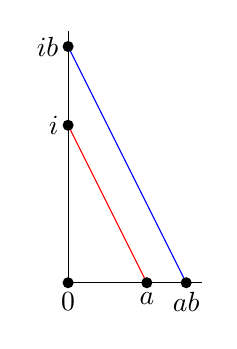
\begin{tikzpicture}
        \coordinate (I) at (0,2);
        \coordinate (A) at (1,0);
        \coordinate (IB) at (0,3);
        \coordinate (AB) at (1.5,0);
        \draw[black] (0,0) -- (0,3.2);
        \draw[black] (0,0) -- (1.7,0);
        \draw[red] (I) -- (A);
        \draw[blue] (IB) -- (AB);
        \fill[black] (I) circle (2pt) node[left] {\(i\)};
        \fill[black] (IB) circle (2pt) node[left] {\(ib\)};
        \fill[black] (A) circle (2pt) node[below] {\(a\)};
        \fill[black] (AB) circle (2pt) node[below] {\(ab\)};
        \fill[black] (0,0) circle (2pt) node[below] {\(0\)};
    \end{tikzpicture}$$
    Addition von Winkeln:
    $$\begin{tikzpicture}
        \coordinate (N) at (0,0);
        \coordinate (E) at (4,0);
        \coordinate (Z) at (4*0.923,4*0.382);
        \coordinate (W) at (4*0.623,4*0.781);
        \coordinate (W') at (4*0.276,4*0.961);
        \coordinate (yE) at (0,4);
        \draw[name path=xAchse] (0,0) -- (4,0);
        \draw[name path=yAchse] (0,0) -- (0,4);
        \draw[name path=erste]  (0,0) -- (Z);
        \draw[name path=zweite] (0,0) -- (W);
        \draw[name path= dritte] (0,0) -- (W');
        \draw[green] (W) -- (4.053,3.127) node[midway, above] {\(|z-1|\)};
        \pic [draw, black, "\( \)", angle radius=4cm, angle eccentricity=1] {angle = E--N--yE};
        \pic [draw, red, "\(\alpha \)", angle radius=1.8cm, angle eccentricity=0.7] {angle = E--N--Z};
        \pic [draw, blue, "\( \beta\)", angle radius=2.5cm, angle eccentricity=0.9] {angle = E--N--W};
        \pic [draw, purple, "\( \alpha\)", angle radius=1.8cm, angle eccentricity=0.8] {angle = W--N--W'};
        \draw[name path=mycircleP, green] (W) circle (4*0.39cm);
        \fill[black] (E) circle (2pt) node[below] {\(1\)};
        \fill[black] (Z) circle (2pt) node[right] {\(z\)};
        \fill[black] (W) circle (2pt) node[left] {\(w\)};
        \fill[purple] (W') circle (2pt) node[above left] {\(w'\)};
     \end{tikzpicture}$$
\end{proof}
\begin{Bem}
    Sei \(0,1\in M\). Dann ist \(\QQ(M\cup\bar M)\subseteq K(M)\).
\end{Bem}
\begin{Satz}[Konstruierbare Zahlen]
    Sei \(0,1\in M\) und \(a\in \CC\). Es gilt
    \begin{align*} a\in K(M)\iff\exists\ \QQ(M\cup\bar M)=K_0\subseteq K_1\subseteq\dots\subseteq K_r \text{ mit }[K_i:K_{i-1}]=2 \text{ und }a\in K_r.
    \end{align*}
    Insbesondere ist \([\QQ(M\cup\bar M\cup\Set{a}):\QQ(M\cup\bar M)]\) eine Zweierpotenz, das heißt \(a\) ist algebraisch über \(\QQ(M\cup\bar M)\).
\end{Satz}
\begin{proof}
    Kurzform: Schnitt von Geraden vergrößert den Körper nicht. Schnitt von Geraden mit Kreisen führt auf quadratische Gleichung. Das heißt \(K_i/K_{i-1}\) hat Grad 2. Das zeigt: \(a\in K(M)\) impliziert, dass eine Kette wie im Satz existiert.
    Zeige: Wenn \(L/K\) eine quadratische Erweiterung ist mit \(L\subseteq \CC\) und \(K\subseteq K(M)\) dann ist auch \(L\subseteq K(M)\).
    Sei \(L=K(b)\) wobei \(b\) eine Nullstelle von \(X^2+cX+d\) ist. Die Substitution \(X=X-\frac{c}{2}\) erreicht \(c=0\). Also sei ohen Einschränkung das Polynom \(X^2+d\) und \(b'=\sqrt{d'}\). Zeige also: Quadratwurzeln in \(\CC\) sind konstruierbar. Es ist \(z=|z|\cdot\frac{z}{|z|}\). Zeige also: Wurzeln aus reellen Zahlen und Winkelhalbierungen sind konstruierbar.
    $$\begin{tikzpicture}
        \coordinate (N) at (0,0);
        \coordinate (A') at (2,1);
        \coordinate (A) at (0.5,2);
        \coordinate (AA') at (2.5,3);
        \draw[black] (N) -- (A);
        \draw[black] (N) -- (A');
        \draw[red] (A) -- (AA');
        \draw[red] (A') -- (AA');
        \draw[name path=L1,blue] (N) -- (AA');
         \fill[black] (A) circle (2pt) node[above left] {\(a\)};
          \fill[black] (A') circle (2pt) node[ right] {\(a'\)};

    \end{tikzpicture}$$
    Sei \(a\in\RR\) und \(a\geq 0\).
    $$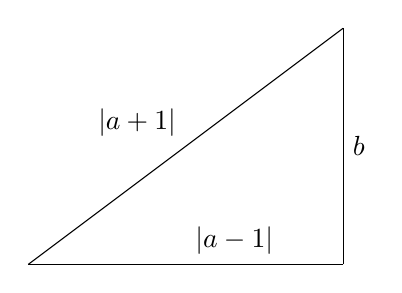
\begin{tikzpicture}
        \draw[black] (0,0) -- (4,0) node[midway, above right] {\(|a-1|\)};
        \draw[black] (4,0) -- (4,3) node[midway, right] {\(b\)};
        \draw[black] (0,0) -- (4,3) node[midway, above left] {\(|a+1|\)};
    \end{tikzpicture}$$
    \begin{align*}
        b^2&=(a+1)^2-(a-1)^2\\
        &=4a
    \end{align*} also \(b=2\sqrt{a}\)
\end{proof}
\begin{Lemma}\label{Lem:KompQuad}
    Sei \(K\) ein Körper und \(K=K_0\subseteq K_1\dots\subseteq K_n\), \(K=L_0\subseteq L_1\dots\subseteq L_m\) Ketten quadratischer Körpererweiterungen.
    Dann ist \(K=L_0\subseteq \dots\subseteq L_m\subseteq K_1L_m\subseteq\dots \subseteq K_nL_m\) Kette höchstens quadratischer Körpererweiterungen.
\end{Lemma}
\begin{proof}
    Es ist \([K_iL_n:K_{i-1}L_n]\leq [K_i:K_{i-1}]=2\)
\end{proof}
\begin{Satz}
    Sei \(K\) ein Körper der Charakterisitik \(\neq 2\) und \(a\in\bar K\). Dann sind äquivalent:
    \begin{enumerate}
        \item Es gibt Kette quadratischer Erweiterungen \(K=K_0\subseteq \dots\subseteq K_n\) and \(a\in K_n\)
        \item Es gibt Galoiserweiterung \(L/K\) mit \(a\in L\) und \([L:K]=2^r\).
    \end{enumerate}
\end{Satz}
\begin{proof}
    Gelte \(1\) und sei \(K_n/K\) gegeben. Dann ist \(K_n/K\) ist separabel und nach \hyperref[Satz:PrimElt]{Satz vom primitiven Element \ref{Satz:PrimElt}} gilt \(K_n=K(b)\) für ein \(b\in K_n\). Sei \(L/K\) die normale Hülle von \(K_n/K\). Nach Konstruktion ist \(L/K\) der Zerfällungskörper vom Minimalpolynom \(f\) von \(b\). Seien \(b_1,\dots,b_n\) die Nullstellen von \(f\) in \(L\) mit \(b=b_1.\) Es ist \(L=K(b_1)\cdots K(B_n)\) Komposition. Da \(f\) das Minimalpolynom von \(b_i\) ist, ist \(K_n=K(b)=K(b_i)\) für alle \(i\) und somit ist \(K(b_i)/K\) durch Kette quadratischer Erweiterungen erreichbar. Nach \hyperref[Lem:KompQuad]{Lemma \ref{Lem:KompQuad}} ist \(L\) als Kompositum durch quadratische Kette erreichbar. Gelte 2. und sei \(L/K\) Galoisch vom Grad \(2^r\). Dann ist \(G=\Gal(L/K)\) eine \(p\)-Gruppe für \(p=2\).
    \(G\) ist auflösbar somit gibt es nach \hyperref[Kor:NormIndex]{Korollar \ref{Kor:NormIndex}} eine normale Untergruppe \(H\subseteq G\) mit \([G:H]=2\).
    Sei \(K_r=L\) und \(K_1=L^H\). Dann ist \([K_1:K_0]=2\) und \(K_r/K\) Galoisch von Grad \(2^{r-1}\). Also folgt die Aussage nach Induktion.
\end{proof}
\begin{Satz}
    \(\pi\in\RR\) ist transzendent über \(\QQ\).
\end{Satz}
\begin{Kor}
    \(\pi\not\in K(0,1)\) da \([\QQ(\pi):\QQ]=\infty\).
\end{Kor}
\begin{Kor}
    Wäre Winkeldrittelung immer möglich, so wäre \(\zeta_9\in K(0,1)\).
    $$\begin{tikzpicture}
        \coordinate (ME) at (-4,0);
        \coordinate (E) at (4,0);
        \coordinate (N) at (0,0);
        \coordinate (S) at (-0.5*4,0.866*4);
        \coordinate (Z) at (0.766*4, 0.642*4); 
        \draw (ME) -- (E);
        \draw[blue] (N) -- (S);
        \draw[blue] (ME) -- (S);
        \draw[blue] (ME) -- (N);
        \draw (N) -- (0,4);
        \draw[purple] (N) -- (Z);
        
        \pic [draw, "\( \)", angle radius=4cm, angle eccentricity=0.8] {angle = E--N--ME};
        \fill[purple] (Z) circle (2pt) node[above right] {\(\zeta_9\)};
        
    \end{tikzpicture}$$
    Aber \([\QQ(\zeta_9):\QQ]=6\) ist keine Zweierpotenz also Widerspruch und die Aussage ist falsch.
\end{Kor}
\begin{Kor}[Würfelverdoppelung]
Ist \(\sqrt[3]{2}\in K(0,1)\)? Es ist \[[\QQ(\sqrt[3]{2}):\QQ]=3\] keine Zweierpotenz, also nein.
    
\end{Kor}
\begin{Def}
    \begin{enumerate}
        \item[]
        \item Ein Körper \(L\) heißt quadratische abgeschlossen, wenn jedes quadratische Polynom in \(L[X]\) in \(L\) eine Nullstelle hat.
        \item Ein quadratischer Abschluss von \(K\) ist eine Erweiterung \(L/K\) sodass \(L\) quadratisch abgeschlossen ist und jede endliche Zwischenerweiterung \(L/L'/K\) lässt sich durch Kette quadratischer Erweiterungen erreichen.
    \end{enumerate}
\end{Def}
\begin{Bem}[Konstruktion eines quadratische Abschluss]
    Sei \[L=\set{a\in\bar K}{ K(a)/K \text{ ist durch Kette quadratischer Erweiterungen erreichbar }}.\]
    Wir haben gesehen: \(K(M)\) ist der quadratische Abschluss von \(\QQ(M\cup\bar M)\)
\end{Bem}
\subsection{Konstruktion des regulären \(n\)-Ecks}
Sei \(E\) die Menge der Ecken des regulären \(n\)-Ecks mit \(E\subseteq S^1=\set{z\in\CC}{ |z|=1}\). Es gilt \(E=\mu_n(\CC)\).
Sei \(\zeta_n\in\mu_n(\CC)\) primitiv. Ist \(\zeta_n\in K(0,1)\)?
Bekannt ist: \([Q(\zeta_n)/\QQ]\) ist Galoisch mit \(G=\Gal(\QQ(\zeta_n)/\QQ)=(\ZZ/n\ZZ)^*\) und \(|G|=\varphi(n)\).
Antwort: \[\zeta_n\in K(0,1)\iff \varphi(n)=2^r.\]
Wenn \(n=\prod_ip_i^{e_i}\) für verschiedene Primzahlen \(p_i\), dann ist \(\varphi(n)=\prod(p_i-1)p_i^{e_i-1}\). Das ist Zweierpotenz genau dann wenn \(e_i<2\) für \(p_i\neq 2\) und \(e_i=1\) nur wenn \(p_i-1\) eine Zweierpotenz ist.
\begin{Def}[Fermatsche Primzahl]
    Eine Fermatsche Primzahl ist eine Primzahl der Form \(p=2^m+1\).
\end{Def}
\begin{Bem}
    Wenn \(p\) prim dann ist \(\zeta_p\) konstruierbar \(\iff p\) ist Fermatsche Primzahl
\end{Bem}
\begin{Lemma}
    \(2^m+1\) prim \(\implies m=2^r\)
\end{Lemma}
\begin{proof}
    Sei \(m=qm'\) wobei \(q\) ungerade. Dann ist nach geometrischer Summe
    \[\dfrac{2^m+1}{2^{m'}+1}=\dfrac{1-(-2^{m'})^q}{1-(-2^{m'})}=\sum_{k=0}^{q-1}(-2^{m'})^k=\sum_{k=1}^q(-1)^{k+1}2^{m-km'}\] also \(2^{m}+1\) nicht prim.
\end{proof}
\begin{Bem}
    \(2^{2^r}+1\) ist prim für \(r=0,1,2,3,4\) aber für \(2^{2^5}+1=641\cdot 6700417\)
\end{Bem}
\begin{Bem}
    Fazit: Reguläre \(3,5,17\) Eck ist konstruierbar. Reguläre \(7,11,13,19\)-Eck nicht.
\end{Bem}
\begin{Bsp}
Sei \(\alpha=\frac{2\pi}5\) und \(\beta=\frac{\pi-\alpha}2=\frac{3\pi}{16}\) und \(\gamma=2\beta=\frac 3 5\pi\)
$$\begin{tikzpicture}
    \coordinate (E1) at (4*0.951,4*0.309);
    \coordinate (E2) at (4*0,4*1);
    \coordinate (E3) at (-4*0.951,4*0.309);
    \coordinate (E4) at (-4*0.588,-4*0.809);
    \coordinate (E5) at (4*0.588, -4*0.809);
    \coordinate (N) at (0,0);
    \draw[name path=K1] (E1) -- (E2);
    \draw[name path=K2] (E2) -- (E3);
    \draw[name path=K3] (E3) -- (E4);
    \draw[name path=K4] (E4) -- (E5);
    \draw[name path=K5] (E5) -- (E1);
    \draw[red] (0,0) -- (E2);
    \draw[red] (0,0) -- (E3);
    \pic [draw, "\(\gamma\)", angle radius=1cm, angle eccentricity=0.5] {angle = E1--E5--E4};
    \pic [draw, "\(\alpha\)", angle radius=1cm, angle eccentricity=0.5] {angle = E2--N--E3};
    \pic [draw, "\(\beta\)", angle radius=1cm, angle eccentricity=0.5] {angle = E3--E2--N};
    \pic [draw, "\(\beta\)", angle radius=1cm, angle eccentricity=0.5] {angle = N--E3--E2};

    
 \end{tikzpicture}$$
 Sei weiter \(\delta=\frac{\pi-\gamma}2\).
 Dann ist \(\delta=\frac{1}{5}\pi\) und \(\gamma-2\delta=\frac 1 5\pi=\delta\)
 $$\begin{tikzpicture}
    \coordinate (E1) at (4*0.951,4*0.309);
    \coordinate (E2) at (4*0,4*1);
    \coordinate (E3) at (-4*0.951,4*0.309);
    \coordinate (E4) at (-4*0.588,-4*0.809);
    \coordinate (E5) at (4*0.588, -4*0.809);
    \coordinate (N) at (0,0);
    \coordinate (F) at (1.454,-0.473);
    \draw[name path=K1] (E1) -- (E2) node[midway,above]{\(1\)};
    \draw[name path=K2] (E2) -- (E3) node[midway,above]{\(1\)};
    \draw[name path=K3] (E3) -- (E4) node[midway, below left]{\(1\)};
    \draw[name path=K4] (E4) -- (E5);
    \draw[name path=K5] (E5) -- (E1);
    \draw[name path=D,red] (E2) -- (E4) node[midway, above left] {\(d\)};
    \draw[name path=EO,red] (E2) -- (F) node[pos=0.6, below left] {\(1\)};
    \draw[name path=EU,red] (E5) -- (F) node[pos=0.6, below left] {\(e\)};
    \draw[blue] (E1) -- (F);
    \pic [draw, "\(\delta\)", angle radius=1cm, angle eccentricity=0.65] {angle = E3--E2--E4};
    \pic [draw, "\(\delta\)", angle radius=1cm, angle eccentricity=0.65] {angle = E4--E2--E5};
    \pic [draw, "\(\delta\)", angle radius=1cm, angle eccentricity=0.65] {angle = E5--E2--E1};
    \pic [draw, "\(2\delta\)", angle radius=1cm, angle eccentricity=0.65] {angle = E5--E4--E2};
    \pic [draw, "\(2\delta\)", angle radius=1cm, angle eccentricity=0.65] {angle = E2--E5--E4};
    \pic [draw, "\(\delta\)", angle radius=1cm, angle eccentricity=0.65] {angle = E1--E5--E2};
    \pic [draw, "\(3\delta\)", angle radius=1cm, angle eccentricity=0.65] {angle = E5--F--E1};
    \pic [draw, "\(2\delta\)", angle radius=1cm, angle eccentricity=0.65] {angle = E1--F--E2};
    \pic [draw, "\(2\delta\)", angle radius=1cm, angle eccentricity=0.65] {angle = E2--E1--F};
    \pic [draw, "\(\delta\)", angle radius=1cm, angle eccentricity=0.65] {angle = F--E1--E5};
    \fill[green] (-2.5,0.7) circle (0pt) node[above] {\(A\)};
    \fill[green] (0,-0.7) circle (0pt) node[above] {\(B\)};
    \fill[green] (2.8,-1) circle (0pt) node[above] {\(C\)};
    \fill[green] (1.6,1.6) circle (0pt) node[above] {\(D\)};

    
 \end{tikzpicture}$$
 Die Dreiecke \(A\) und \(C\) sind ähnlich und die Dreiecke \(B\) und \(D\) sind ähnlich, da sie gleiche Winkel haben.
 Sei \(d\) die Länge der Diagonalen und \(e=d-1\)
 Es gilt also \(\frac 1 d=\frac{1}{e}=\frac{1}{d-1}\)
 Also ist \(d^2-d=1\) was \(d=\dfrac{\sqrt 5+1}{2}\) impliziert.
 Konstruiere also
 $$\begin{tikzpicture}
     \coordinate (N) at (0,0);
     \coordinate (E) at (4,0);
     \coordinate (F) at (4,2);
     \draw (N) -- (E) node[midway, below]{\(1\)};
     \draw (E) -- (F) node[midway, right]{\(\frac 1 2\)};
     \draw (N) -- (F) node[midway, above]{\(\frac{\sqrt 5}{2}\)};
 \end{tikzpicture}$$
 und dann konstruiere 5-Eck.
\end{Bsp}
\subsection{Auflösbarkeit durch Radikale}
\begin{Def}
    Sei \(K\) ein Körper der Charakteristik 0.
    \begin{enumerate}
        \item Eine einfache Radikalerweiterung ist eine Körpererweiterung \(L/K\) sodass \(L=K(a)\) für ein \(a\) mit \(a^n\in K\) für ein \(n\in\NN_1\)
        \item \(L/K\) heißt Radikalerweiterung, wenn es eine Kette \(K=K_0\subseteq\dots \subseteq K_r=L\) gibt sodass \(K_i/K_{i-1}\) eine einfache Radikalerweiterung ist.
        \item \(L/K\) ist auflösbar durch Radikale, wenn es für jedes \(a\in L\) eine Radikalerweiterung \(L'/K\) und Einbettung \(K(a)\subseteq L'\) existiert.
    \end{enumerate}
\end{Def}
\begin{Bem}
    Wenn \(L/K\) endlich, dann ist \(L=K(a)\) für ein \(a\in L\).
    Dann
    \[L/K \text{ ist auflösbar durch Radikale}\iff L\text{ ist in einer Radikalerweiterung enthalten}\]
\end{Bem}
\begin{Bem}
    Notation: Wenn \(L/K\) einfache Radikalerweiterung, \(L=K(a)\) und \(a\) Nullstelle von \(X^n-b\) könnte schreiben \(a=\sqrt[n]{b}\) aber das ist ungenau da \(X^n-b\) \(n\) verschiedene Nullstellen hat.
\end{Bem}
\begin{Bsp}
    Sei \(f=X^3-2\) und sei \(a=\sqrt[3]{2}\in\RR\). Wenn \(K=\QQ(a)\) dann ist \([K(a):K]=1\) aber \([K(\zeta_3 a):K]=2\)
\end{Bsp}
\begin{Bem}
    Angenommen \(K\) ist ein Körper von Charakteristik \(\neq n\) und \(\mu_n(\bar K)\subseteq K\) Dann sei \(\zeta_n\in\mu_n(\bar K)\) primitiv.
    Die Nullstellen von \(f=X^n-b\) sind \(a,\zeta_na,\zeta_n^2a,\dots,\zeta_n^{n-1}a\) also 
    \(X^n-b=\prod\limits_{k=0}^{n-1}(X-\zeta_n^ka)\) und \(K(a)=K(\zeta_n^ka)\) für jedes \(k\) da \(K\) \(\zeta_n\) enthält. In diesem Fall ist die Bezeichnung \(K(\sqrt[n]{b})=K(a)\) für irgendein \(a\) mit \(a^n=b\). Das ist ein Zerfallskörper von \(X^n-b\).
\end{Bem}
\begin{Lemma}\label{Lem:EinfRadZykl}
    Sei \(K\) ein Körper der Charakteristik \(\neq n\) und \(\mu_n(\bar K)\subseteq K\). Dann gibt es einen injektiven Gruppenhomomorphismus \(\Gal(K(\sqrt[n]{a})/K)\to \mu_n(K)\cong \ZZ/n\ZZ\). Insbesondere ist \(G=\Gal(L/K)\) zyklisch.
\end{Lemma}
\begin{proof}
    Sei \(\sigma\in G\) und \(b=\sqrt[n]{a}\). Es ist \(\sigma(b)\) ist eine Nullstelle von \(X^n-a\) also ist \(\sigma(b)=\zeta b\) für ein \(\zeta\in\mu_n(K)\).
    Da \(\mu_n(\bar K)\subseteq K\) ist für \(\zeta'\in\mu_n(\bar K):\)
    \[\sigma(\zeta'b)=\zeta'\sigma(b)=\zeta'\zeta b.\]
    Sei \(\psi\colon G\to \mu_n(\bar K), \ \psi(\sigma)=\frac{\sigma(b)}{b}\). Eine Rechnung zeigt, dass das ein Gruppenhomomorphismus ist. Angenommen \(\psi(\sigma)=1\).
    Dann ist \(\sigma=\id\) auf Menge der Nullstellen und da \(K(\sqrt[n]{a})/K\) Zerfällungskörper ist, ist \(\sigma=\id\).
\end{proof}
\begin{Def}
    Sei \(E\) eine Eigenschaft von Gruppen (z.B. zyklisch, auflösbar, abelsch...) Eine Körpererweiterung \(L/K\) hat die Eigenschaft \(E\), wenn \(L/K\) Galoisch ist und \(\Gal(L/K)\) diese Eigenschaft \(E\) hat.
\end{Def}
\begin{Satz}\label{Satz:ZyklWurzel}
    Sei \(Char(K)\neq n\) und \(\mu_n(\bar K)\subseteq K\). Wenn \(L/K\) zyklisch von Grad \(n\), dann ist \(L=K(\sqrt[n]{a})\) für ein \(a\in K\).
\end{Satz}
\begin{proof}
    Sei \(\sigma\in\Gal(L/K)\) ein Erzeuger. Als Endormorphismus gilt \(\sigma^n-\id=0\). Sei \(\mu_\sigma\) Minimalpolynom von \(\sigma\).
    Dann gilt \(\mu_\sigma\mid X^n-1=\prod_{\zeta\in\mu_n}(X-\zeta)\). Somit ist \(\sigma\) diagonalisierbar und die Eigenwerte sind die Nullstellen von \(\mu_\sigma\). Sei \(B\subseteq \mu_n\) die Menge dieser Nullstellen. Für \(\zeta\in \mu_n(\bar K)\) sei \(V_\zeta=\set{x\in L}{ \sigma(x)=\zeta x}\). Es gilt \(V_\zeta\neq 0\iff \zeta\in B\) und
    \(L=\oplus_{\zeta\in\mu_n}V_\zeta\).
    Sei \(x\in V_\zeta\) mit \(x\neq 0\). Dann gilt \(x^{-1}\in V_{\zeta^{-1}}\) und somit haben wir inverse Abbildungen 
    \[V_{\zeta'}\stackrel{x}\to V_{\zeta\zeta'}\stackrel{x^{-1}}\to V_{\zeta'}\] somit ist \(V_{\zeta'}\cong V_{\zeta\zeta'}\)
    Das zeigt: \(B\subseteq \mu_n(\bar K)\) ist Untergruppe und wenn \(\zeta\in B\) Erzeuger ist, dann  ist \(V_1\cong V_\zeta\cong V_{\zeta^2}\cong\dots\).
    Also ist \[\dim(V_{\zeta^i})=\dim(V_1)\] und \(\dim(V_1)=[\mu_n:B]\) denn \(n=\dim(L)=|B|\cdot \dim(V_1)\).
    Es ist 
    \[V_1=\set{x\in L}{ \sigma(x)=x}=L^{\langle \sigma\rangle}=L^G=K\] also \(\dim(V_1)=1\) und somit \(\mu_n=B\) und \(\dim(V_\zeta)=1\) für alle \(\zeta\in\mu_n\).
    Sei \(\zeta_n\in\mu_n\) primitiv. Wähle \(b\in V_{\zeta_n}\) mit \(b\neq 0\). Es ist \(\langle b^i\rangle=V_{\zeta_n^i}\) somit erzeugen \(1,b,\dots, b^{n-1}\) den \(K\)-Vektorraum \(L\). Also ist \(L=K(b)\).
    Es ist \(\sigma(b)=\zeta_nb\) also \(\sigma(b^n)=b^n\) und somit ist \(a=b^n\in L^G=K\). Das zeigt: \(b\) ist Nullstelle von \(X^n-a\in K[X]\)
\end{proof}
\begin{Lemma}
    Die Komposition von Radikalerweiterungen ist eine Radikalerweiterung.
\end{Lemma}\label{Lem:KompRad}
\begin{proof}
    Seien \(K=K_0\subseteq K_1\subseteq \dots \subseteq K_r\) und \(K=L_0\subseteq L_2\subseteq \dots \subseteq L_n\) Ketten von einfachen Radikalerweiterungen.
    Dann ist \(K=K_0\subseteq \dots K_r=K_rL_0\subseteq K_rL_1\subseteq\dots \subseteq K_rL_n\) Kette von einfachen Radikalerweiterungen, denn wenn \(L_i=L_{i-1}(a_i)\) mit \(a_i^n\in L_{i-1}\) dann ist \(K_rL_i=K_rL_{i-1}(a_i)\) und \(a_i^n\in K_rL_{i-1}\)
\end{proof}
\begin{Lemma}\label{Lem:AuflRad}
    Sei \(L/K\) eine endliche Körpererweiterung in Charakterisitk \(0\).
    \begin{enumerate}
        \item \(L/K\) ist Radikalerweiterung \(\implies \) normale Hülle von \(L/K\) ist Radikalerweiterung.
        \item \(L/K\) ist auflösbar durch Radikale \(\iff\) normale Hülle von \(L/K\) ist auflösbar durch Radikale.
    \end{enumerate}
\end{Lemma}
\begin{proof}
    1):Sei \(L=K(a)\) und seien \(a=a_1,\dots,a_r\in\bar K\) die Nullstellen vom Minimalpolynom von \(a\). Also ist die normale Hülle gegeben durch \(M=K(a_1)\cdots K(a_r)\).
    Es ist \(K(a_i)\cong K(a)\) Radikalerweiterung über \(K\). Nach \hyperref[Lem:KompRad]{Lemma \ref{Lem:KompRad}} ist also \(M/K\) eine Radikalerweiterung.\\
    2): Sei \(L=K(a_1)/K\) auflösbar durch Radikale, dh. es gibt \(L'/L\) sodass \(L'/K\) Radikalerweiterung ist. Sei \(M/K\) bzw \(M'/K\) die normale Hülle von \(L/K\) bzw \(L'/K\). Dann ist \(M\subseteq M'\). Nach 1) ist \(M'/K\) Radikalerweiterung also \(M/K\) auflösbar durch Radikale.
    Sei andersrum \(M/K\) die normale Hülle von \(L/K\) und \(M/K\) auflösbar durch Radikale, dh. Es gibt \(M'/M\) sodass \(M'/K\) Radikalerweiterung. Dann ist \(L/K\) auflösbar durch Radikale nach Definition.
\end{proof}
\begin{Satz}
    Sei \(L/K\) endliche Körpererweiterung in Charakteristik \(0\) und \(M/K\) eine normale Hülle. Dann ist \(L/K\) auflösbar durch Radikale \(\iff L/K\) auflösbar.
\end{Satz}
\begin{proof}
    Nach \hyperref[Lem:AuflRad]{Lemma \ref{Lem:AuflRad}} ist ohne Einschränkung \(L/K\) Galoisch.
    Sei \(n=[L:K]\) und \(K'=K(\mu_n)\) und \(L'=L(\mu_n)\).
    Da \(L/K\) Galoisch ist \(L'/K'\) Galoisch und \(L'/K\) Galoisch. Es sind \(\Gal(K'/K)\) und \(\Gal(L'/L)\) abelsch, insbesondere auflösbar.
    Es ist \[\Gal(L/K)\cong \Gal(L'/K)/\Gal(L'/L)\] und \(\Gal(L'/K)/\Gal(L'/K')\cong \Gal(K'/K)\).
    Also ist \begin{align*}
        \Gal(L/K)\text{ auflösbar }&\iff \Gal(L'/K) \text{ auflösbar}\\
        &\iff \Gal(L'/K') \text{ auflösbar}
    \end{align*}
    und \(K'/K\) und \(L'/L\) sind Radikalerweiterungen. Somit ist \(L/K\) auflösbar durch Radikale \(\iff L'/K'\) auflösbar durch Radikale. Somit ist ohne Einschränkung \(L=L'\) und \(K=K'\).
    Sei \(L/K\) auflösbar. Wähle Normalreihe in \(\Gal(L/K)\) mit primzyklischen Quotienten. Das entsprich \(K=K_0\subseteq K_1\subseteq\dots\subseteq K_n=L\) mit \(K_i/K_{i-1}\) Galoisch und \(\Gal(K_i/K_{i-1})\cong \ZZ/p_i\ZZ\).  \hyperref[Satz:ZyklWurzel]{Satz \ref{Satz:ZyklWurzel}} impliziert, dass \(K_i/K_{i-1}\) eine einfache Radikalerweiterung ist. Somit ist \(L/K\) eine Radikalerweiterung. Insbesondere ist \(L/K\) auflösbar durch Radikale.\\
    Sei andersrum \(L/K\) auflösbar durch Radikale. Es gibt \(L'/L\), sodass \(L'/K\) Radikalerweiterung ist. Ohne Einschränkung ist \(L'/K\) Galoisch. Es gibt Kette \(K=K_0\subseteq K_1\subseteq\dots\subseteq K_n=L'\) sodass \(K_i/K_{i-1}\) einfache Radikalerweiterung ist.
    Behauptung: \(\Gal(L'/K)\) ist auflösbar. Dann ist \(\Gal(L/K)\) als Quotient von \(\Gal(L'/K)\) auch auflösbar.
    \hyperref[Lem:EinfRadZykl]{Lemma \ref{Lem:EinfRadZykl}} impliziert, dass \(K_i/K_{i-1}\) Galoisch ist mit zyklischer Galoisgruppe. DIe Körperkette entspricht Kette von Untergruppen in \(\Gal(L'/K)\). Das ist eine abelsche Normalreihe.
\end{proof}
\begin{Kor}
    Jede Gleichung von Grad \(\leq 4\) in Charakterisitk \(0\) ist durch Radikale auflösbar, dh. \(f\in K[X]\) mit \(\deg(f)\leq 4\) und \(L/K\) Zerfällungskörper von \(f\), dann ist \(G=\Gal(L/K)\) auflösbar.
\end{Kor}
\begin{proof}
    Haben injektiven Gruppenhomomorphismus \(G\to S_4\). Da \(S_4\) auflösbar ist, ist \(G\) auflösbar.
\end{proof}
\begin{Satz}
    Für jede endliche Gruppe \(G\) gibt es eine Galoiserweiterung \(L/K\) in Charakteristik \(0\) mit \(G=\Gal(L/K)\).
\end{Satz}
\begin{proof}
    Wähle \(G\to S_n\) injektiv mit \(|n|=G\). Wenn \(L/K'\) existiert mit \(\Gal(L/K')=S_n\) dann gilt für \(K=L^G\) dass \(\Gal(L/K)=G\) ist.
    \(S_n\) operiert auf \(L=\QQ(X_1,\dots,X_n)\) durch Permutation der Variablen. Das gibt Homomorphismus \(S_n\to\Aut(L)\) der injektiv ist. Der Körper \(K=L^{S_n}\) gibt \(\Gal(L/K)=S_n\).
\end{proof}
\begin{Bem}
    \(S_5\) ist nicht auflösbar. 
\end{Bem}
\begin{Bem}
    \begin{enumerate}
        \item[]
        \item Es gibt eine Definition von Auflösbar durch Radikale in beliebiger Charakteristik, für die der letzte Satz gilt
        \item Frage: Wenn \(K\) gegeben, welche Gruppen \(G\) sind als Galoisgruppen über \(K\) realisierbar, dh. gibt es \(L/K\) Galoisch mit \(\Gal(L/K)=G\).
        \begin{enumerate}
            \item \(K=\RR\) Dann ist \(G=\Set{1}\) und \(G=\ZZ/2\ZZ\) möglich.
            \item Wenn \(K\) endlich ist: Genau die zyklischen Gruppen sind möglich, denn \[\Gal(\FF_{q^n}/\FF_q)\cong\langle Fr\rangle\cong\ZZ/n\ZZ.\]
            \item \(K=\QQ\) Frage ist offen. \(G=S_p\) nach Übungsaufgabe?
            \(G=S_n\) möglich (Hilbert).
        \end{enumerate}
    \end{enumerate}
\end{Bem}
\begin{Satz}
    Es gibt Gleichungen vom Grad \(5\) die nicht auflösbar sind
    \end{Satz}
    \begin{proof}
        \(S_5\) ist Galoisgruppe von \(M/\QQ\) für ein \(M/\QQ\) Galoisch. Es ist \(H=S_4=\Stab(1)\subseteq S_5\) also \([G:H]=5\) und somit \([M^H:K]=5\). Es ist \(M=K(a)\) für ein \(a\). Die normale Hülle von \(M^H/K\) entspricht nach Galoiskorrespondenz \(\bigcap_{g\in S_5}gHg^{-1}=\Set{e}\), also ist \(M/K\) die normale Hülle von \(M^H=\QQ(a)=\QQ[X]/(f)\) wobei \(f\) das Minimalpolynom von \(a\) ist. Damit ist \(S_5\) Galoisgruppe von \(f\) und \(S_5\) ist nicht auflösbar. Es ist \(\deg(f)=[\QQ(a):\QQ]=5\)
    \end{proof}